% Unofficial UofT Poster template.
% A fork of the UMich template https://www.overleaf.com/latex/templates/university-of-michigan-umich-poster-template/xpnqzzxwbjzc
% which is fork of the MSU template https://www.overleaf.com/latex/templates/an-unofficial-poster-template-for-michigan-state-university/wnymbgpxnnwd
% which is a fork of https://www.overleaf.com/latex/templates/an-unofficial-poster-template-for-new-york-university/krgqtqmzdqhg
% which is a fork of https://github.com/anishathalye/gemini
% also refer to https://github.com/k4rtik/uchicago-poster

\documentclass[final]{beamer}

% ====================
% Packages
% ====================

\usepackage[T1]{fontenc}
\usepackage[utf8]{luainputenc}
\usepackage{lmodern}
\usepackage[size=custom, width=122,height=91, scale=1.2]{beamerposter}
\usetheme{gemini}
\usecolortheme{uoft}
\usepackage{graphicx}
\usepackage{booktabs}
\usepackage{tikz}
\usepackage{pgfplots}
\pgfplotsset{compat=1.14}
\usepackage{anyfontsize}

% ====================
% Lengths
% ====================

% If you have N columns, choose \sepwidth and \colwidth such that
% (N+1)*\sepwidth + N*\colwidth = \paperwidth
\newlength{\sepwidth}
\newlength{\colwidth}
\setlength{\sepwidth}{0.008\paperwidth}
\setlength{\colwidth}{0.315\paperwidth}

\newcommand{\separatorcolumn}{\begin{column}{\sepwidth}\end{column}}

% ====================
% Title
% ====================

\title{Dataset Distillation: \\ A Data-Efficient Learning Framework}

\author{Swapnil Patel}

\institute[shortinst]{Electrical \& Computer Engineering, University of Toronto}

% ====================
% Footer (optional)
% ====================

\footercontent{
	\href{https://github.com/Swapnil949/ECE1512_2024F_ProjectRepo_SwapnilPatel}{Github: https://github.com/Swapnil949/ECE1512\_2024F\_ProjectRepo\_SwapnilPatel} \hfill
	\href{mailto:swap.patel@mail.utoronto.ca}{swap.patel@mail.utoronto.ca}}
% (can be left out to remove footer)

% ====================
% Logo (optional)
% ====================

% use this to include logos on the left and/or right side of the header:
% Left: institution
\logoleft{
\includegraphics[height=6cm]{figures/ECE_logo.png}}
% Right: funding agencies and other affilations 
%\logoright{\includegraphics[height=7cm]{logos/NSF.eps}}
% ====================
% Body
% ====================
\begin{document}
\begin{columns}
	\separatorcolumn
	\begin{column}{\colwidth}
		\begin{block}{Abstract}
			This project evaluates dataset distillation using DataDAM, creating compact synthetic datasets. MNIST results show efficiency and representativeness, while MHIST was less promising. DataDAM was also compared with PAD, highlighting trade-offs in accuracy and efficiency.
		\end{block}
		\begin{block}{Introduction}
			\begin{figure}[ht]
			\centering
			% First image
			\begin{minipage}{0.49\textwidth}
				\centering
				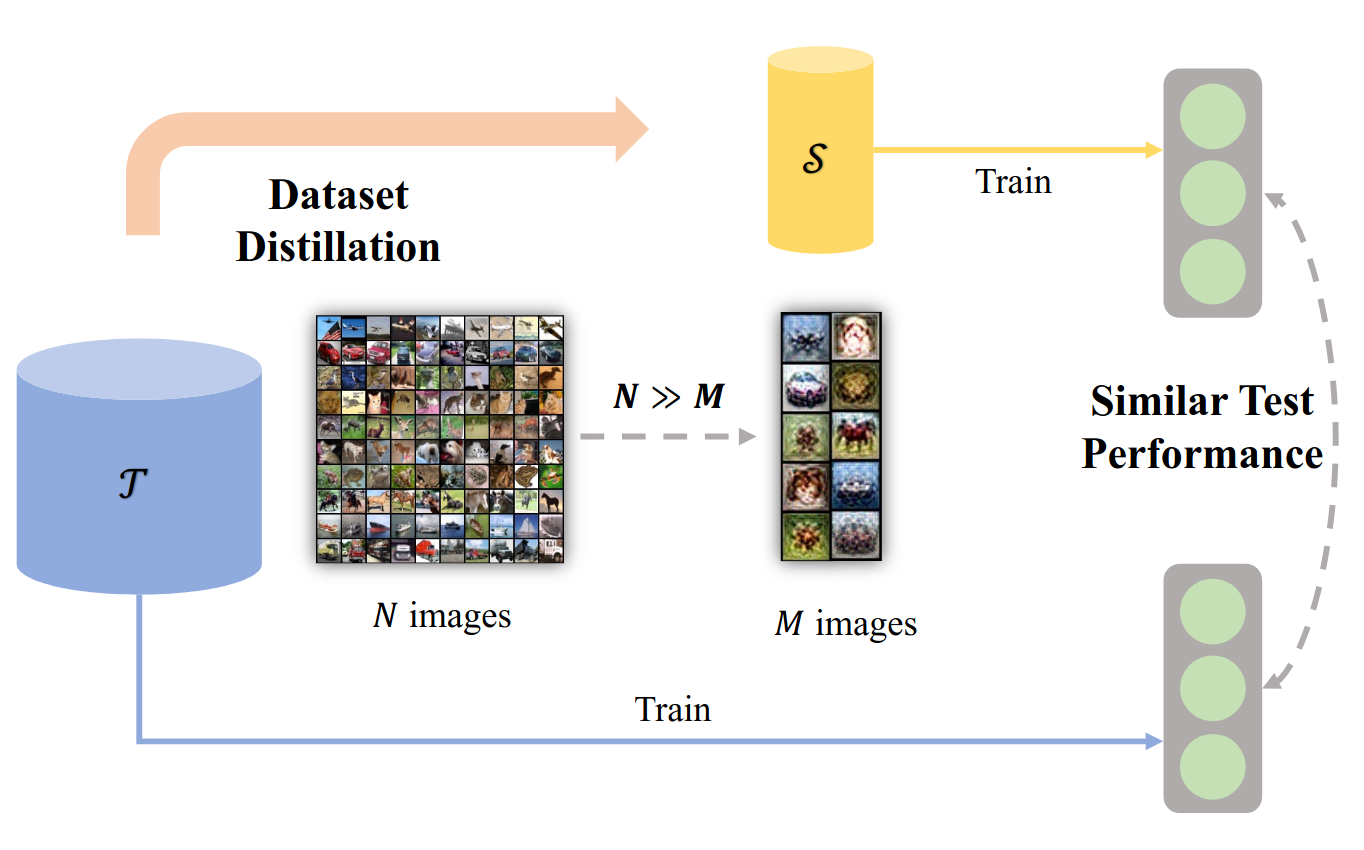
\includegraphics[width=\textwidth]{figures/dataD.png}
				\label{fig:datad}
			\end{minipage}
			\hfill
			% Second image
			\begin{minipage}{0.49\textwidth}
				\centering
				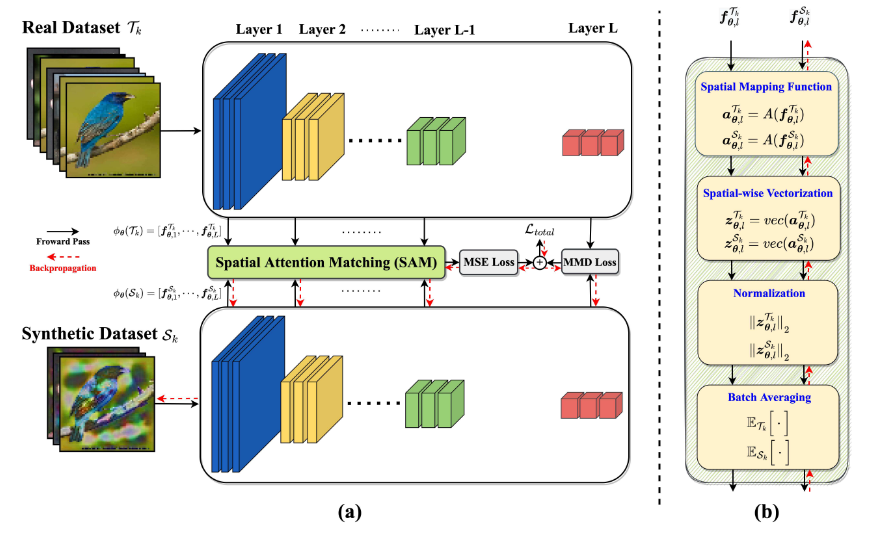
\includegraphics[width=\textwidth]{../report/figures/datadam.png}
				\label{fig:dataDAM}
			\end{minipage}
		\end{figure}
		
		\begin{itemize}
			\item \textbf{Definition:} Dataset distillation is a technique to create compact synthetic datasets that retain the critical information of the original data, enabling efficient model training.
			\item \textbf{Motivation:} As datasets grow in size, training machine learning models becomes computationally expensive. Dataset distillation addresses this by reducing memory and compute requirements without significantly sacrificing performance.
		\end{itemize}
		\textbf{Dataset Distillation with Attention Matching:}
		\begin{itemize}
			\item  Attention Matching focuses on aligning attention maps from real and synthetic datasets across layers of a neural network to capture critical features.
			\item Uses Spatial Attention Mapping (SAM) to extract and align attention distributions.
			\item Employs randomly initialized networks instead of pre-trained ones, enhancing generalization across architectures.
		\end{itemize}
		\end{block}
		
		\begin{block}{Distilled Dataset}
			\begin{figure}[H]
				\centering
				% First image
				\begin{minipage}{0.43\textwidth}
					\centering
					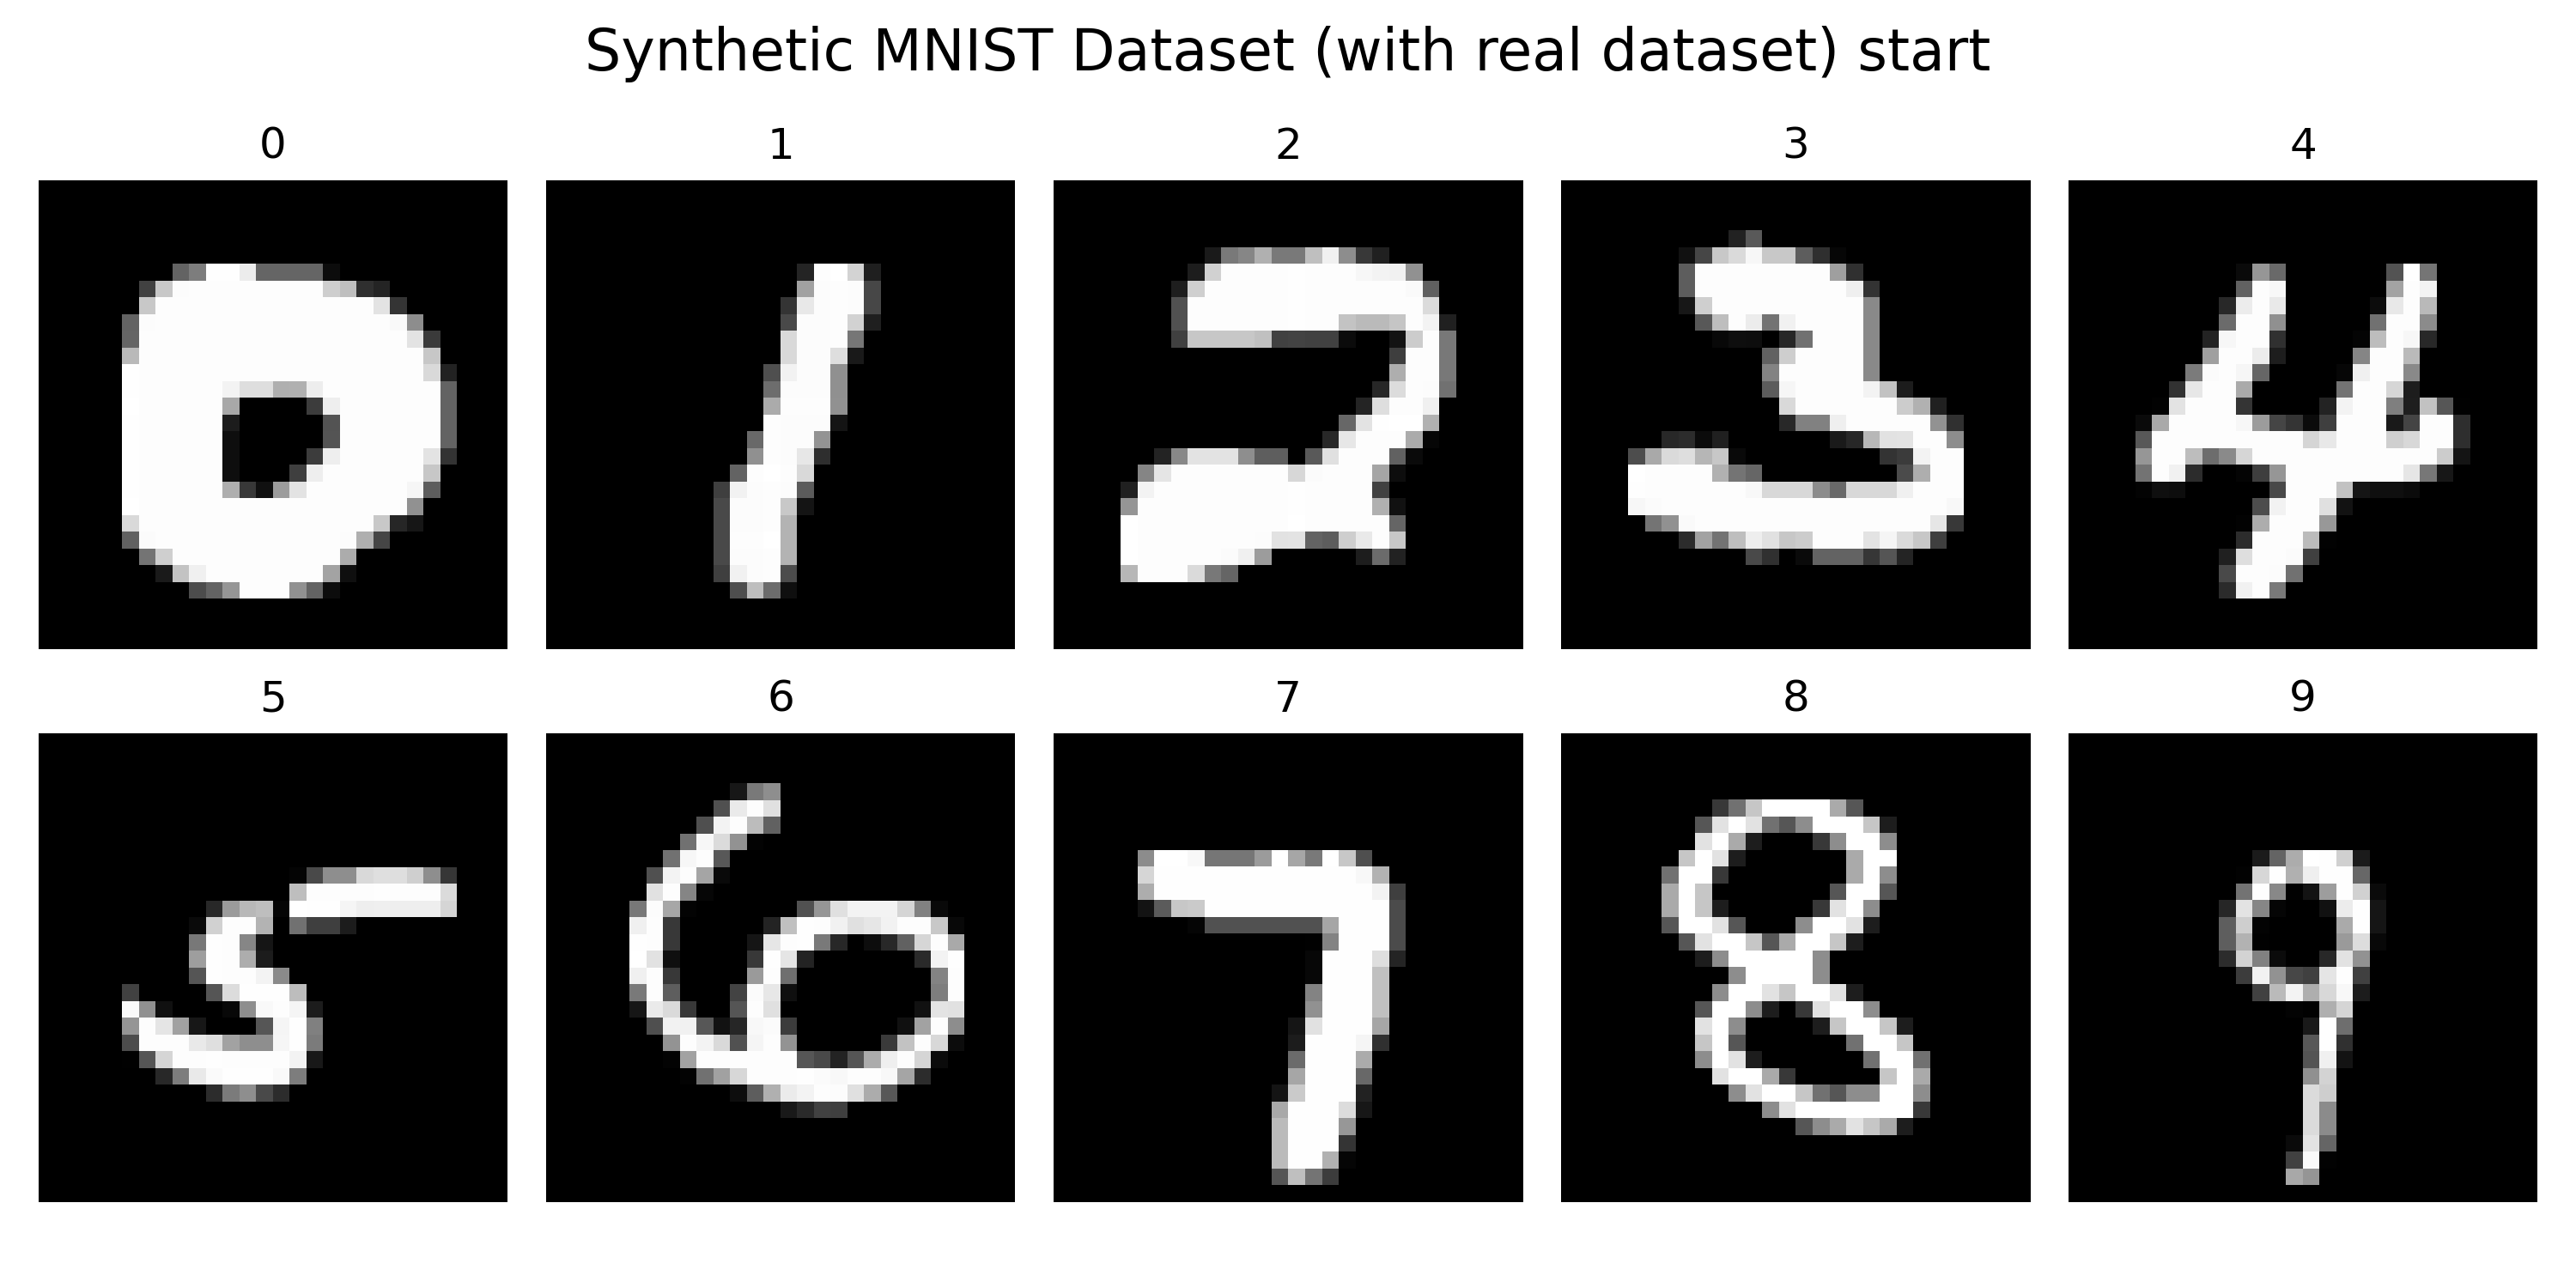
\includegraphics[width=\textwidth]{../report/figures/mnist_real_sample.png}
					\label{fig:mnist-before}
				\end{minipage}
				\hfill
				% Second image
				\begin{minipage}{0.43\textwidth}
					\centering
					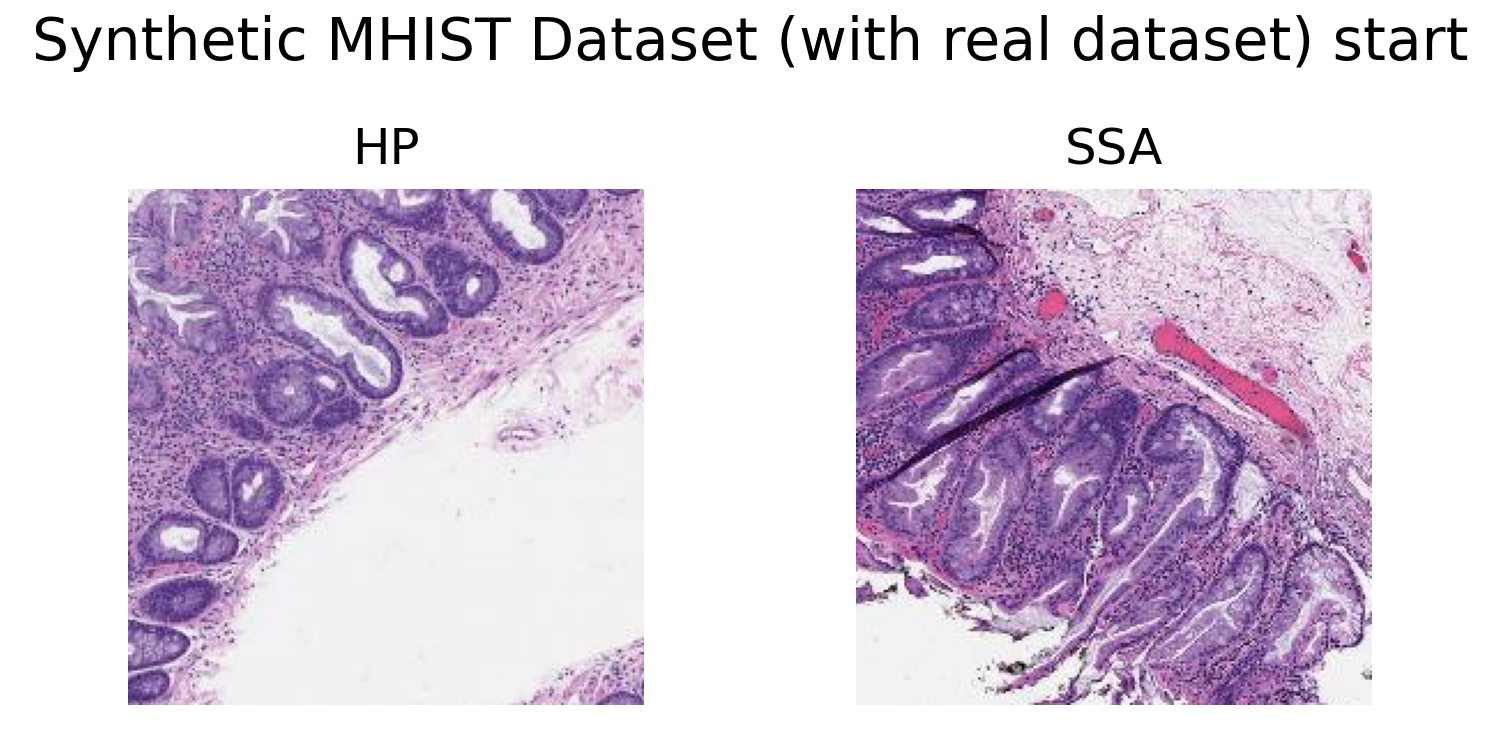
\includegraphics[width=\textwidth]{../report/figures/mhist_real_sample.png}
					\label{fig:mnist-after}
				\end{minipage}
				\label{fig:mnist-comparison}
			\end{figure}
			\begin{figure}[H]
				% First image
				\centering
				\begin{minipage}{0.43\textwidth}
					\centering
					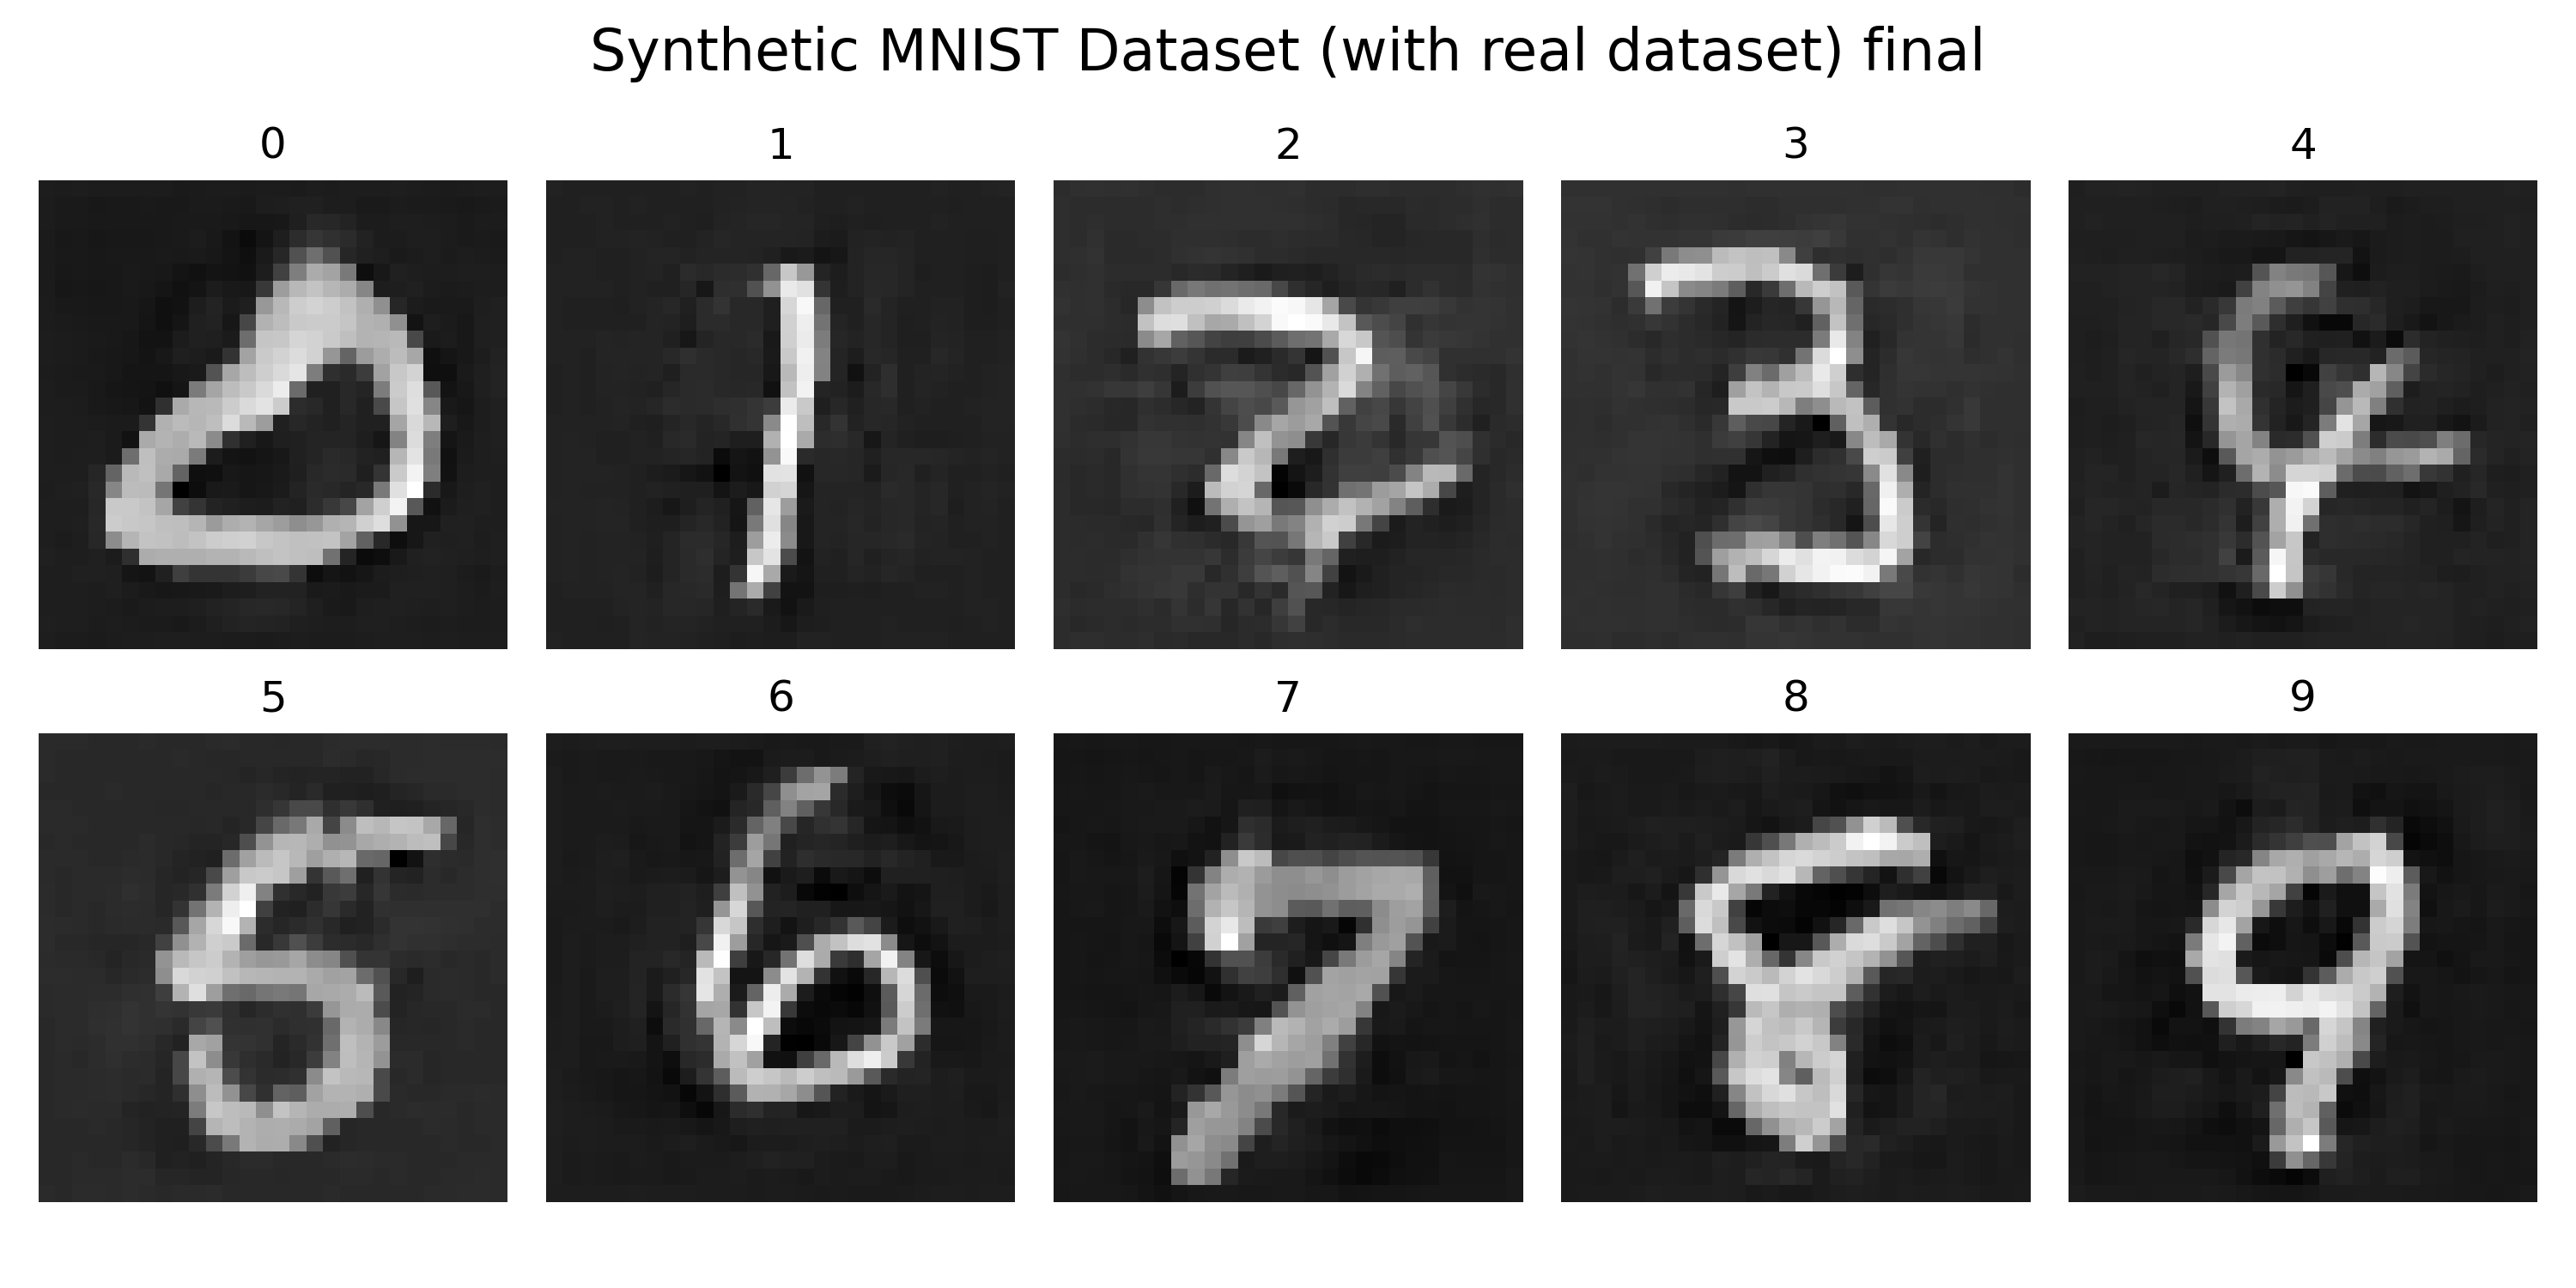
\includegraphics[width=\textwidth]{../report/figures/mnist_real_syn.png}
					\label{fig:mhist-before}
				\end{minipage}
				\hfill
				% Second image
				\begin{minipage}{0.43\textwidth}
					\centering
					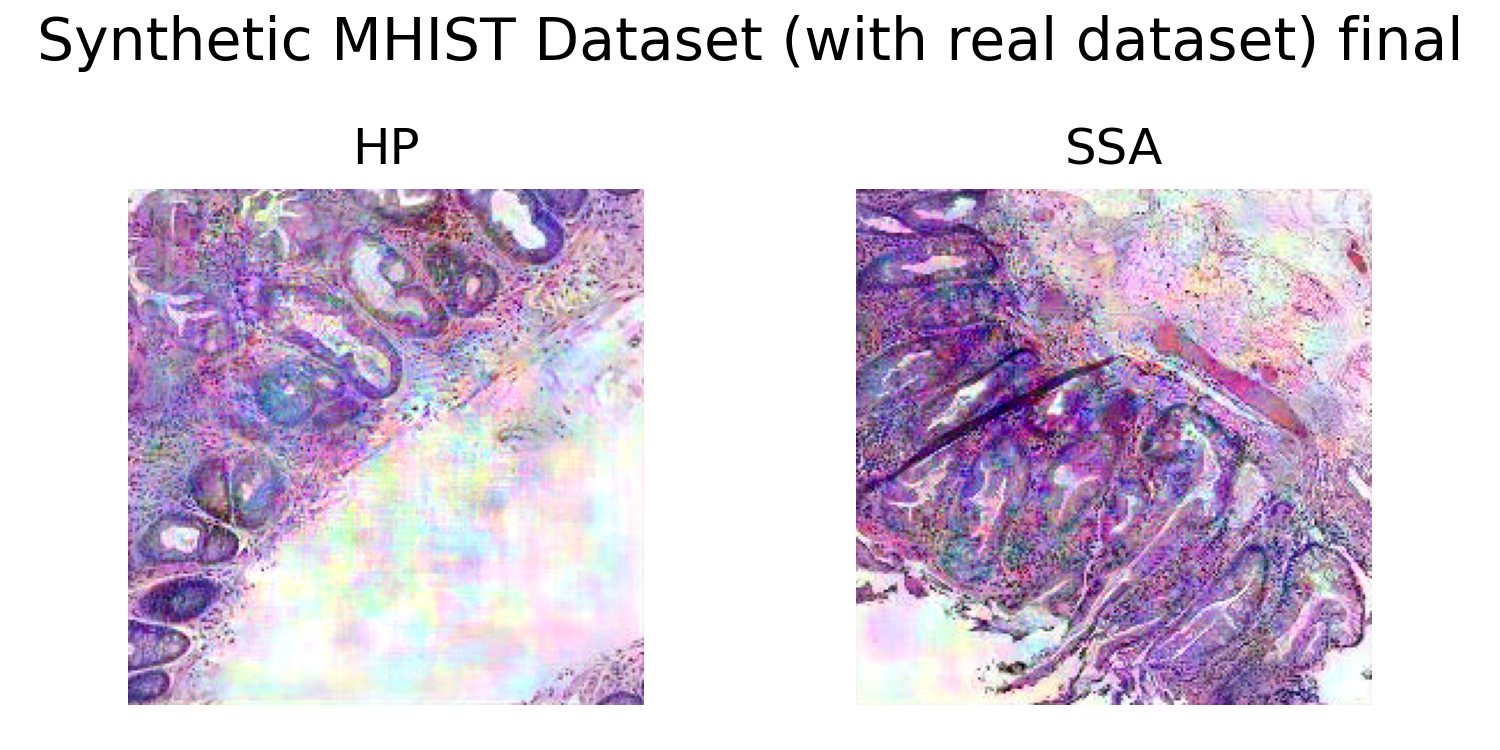
\includegraphics[width=\textwidth]{../report/figures/mhist_real_syn.png}
					\label{fig:mhist-after}
				\end{minipage}
				\label{fig:mhist-comparison}
			\end{figure}
			
		\end{block}
	\end{column}
	\separatorcolumn
	\begin{column}{\colwidth}
		\begin{block}{Synthetic Dataset Evaluation}
			
			\begin{figure}[ht]
				\centering
				% First image
				\begin{minipage}{0.48\textwidth}
					\centering
					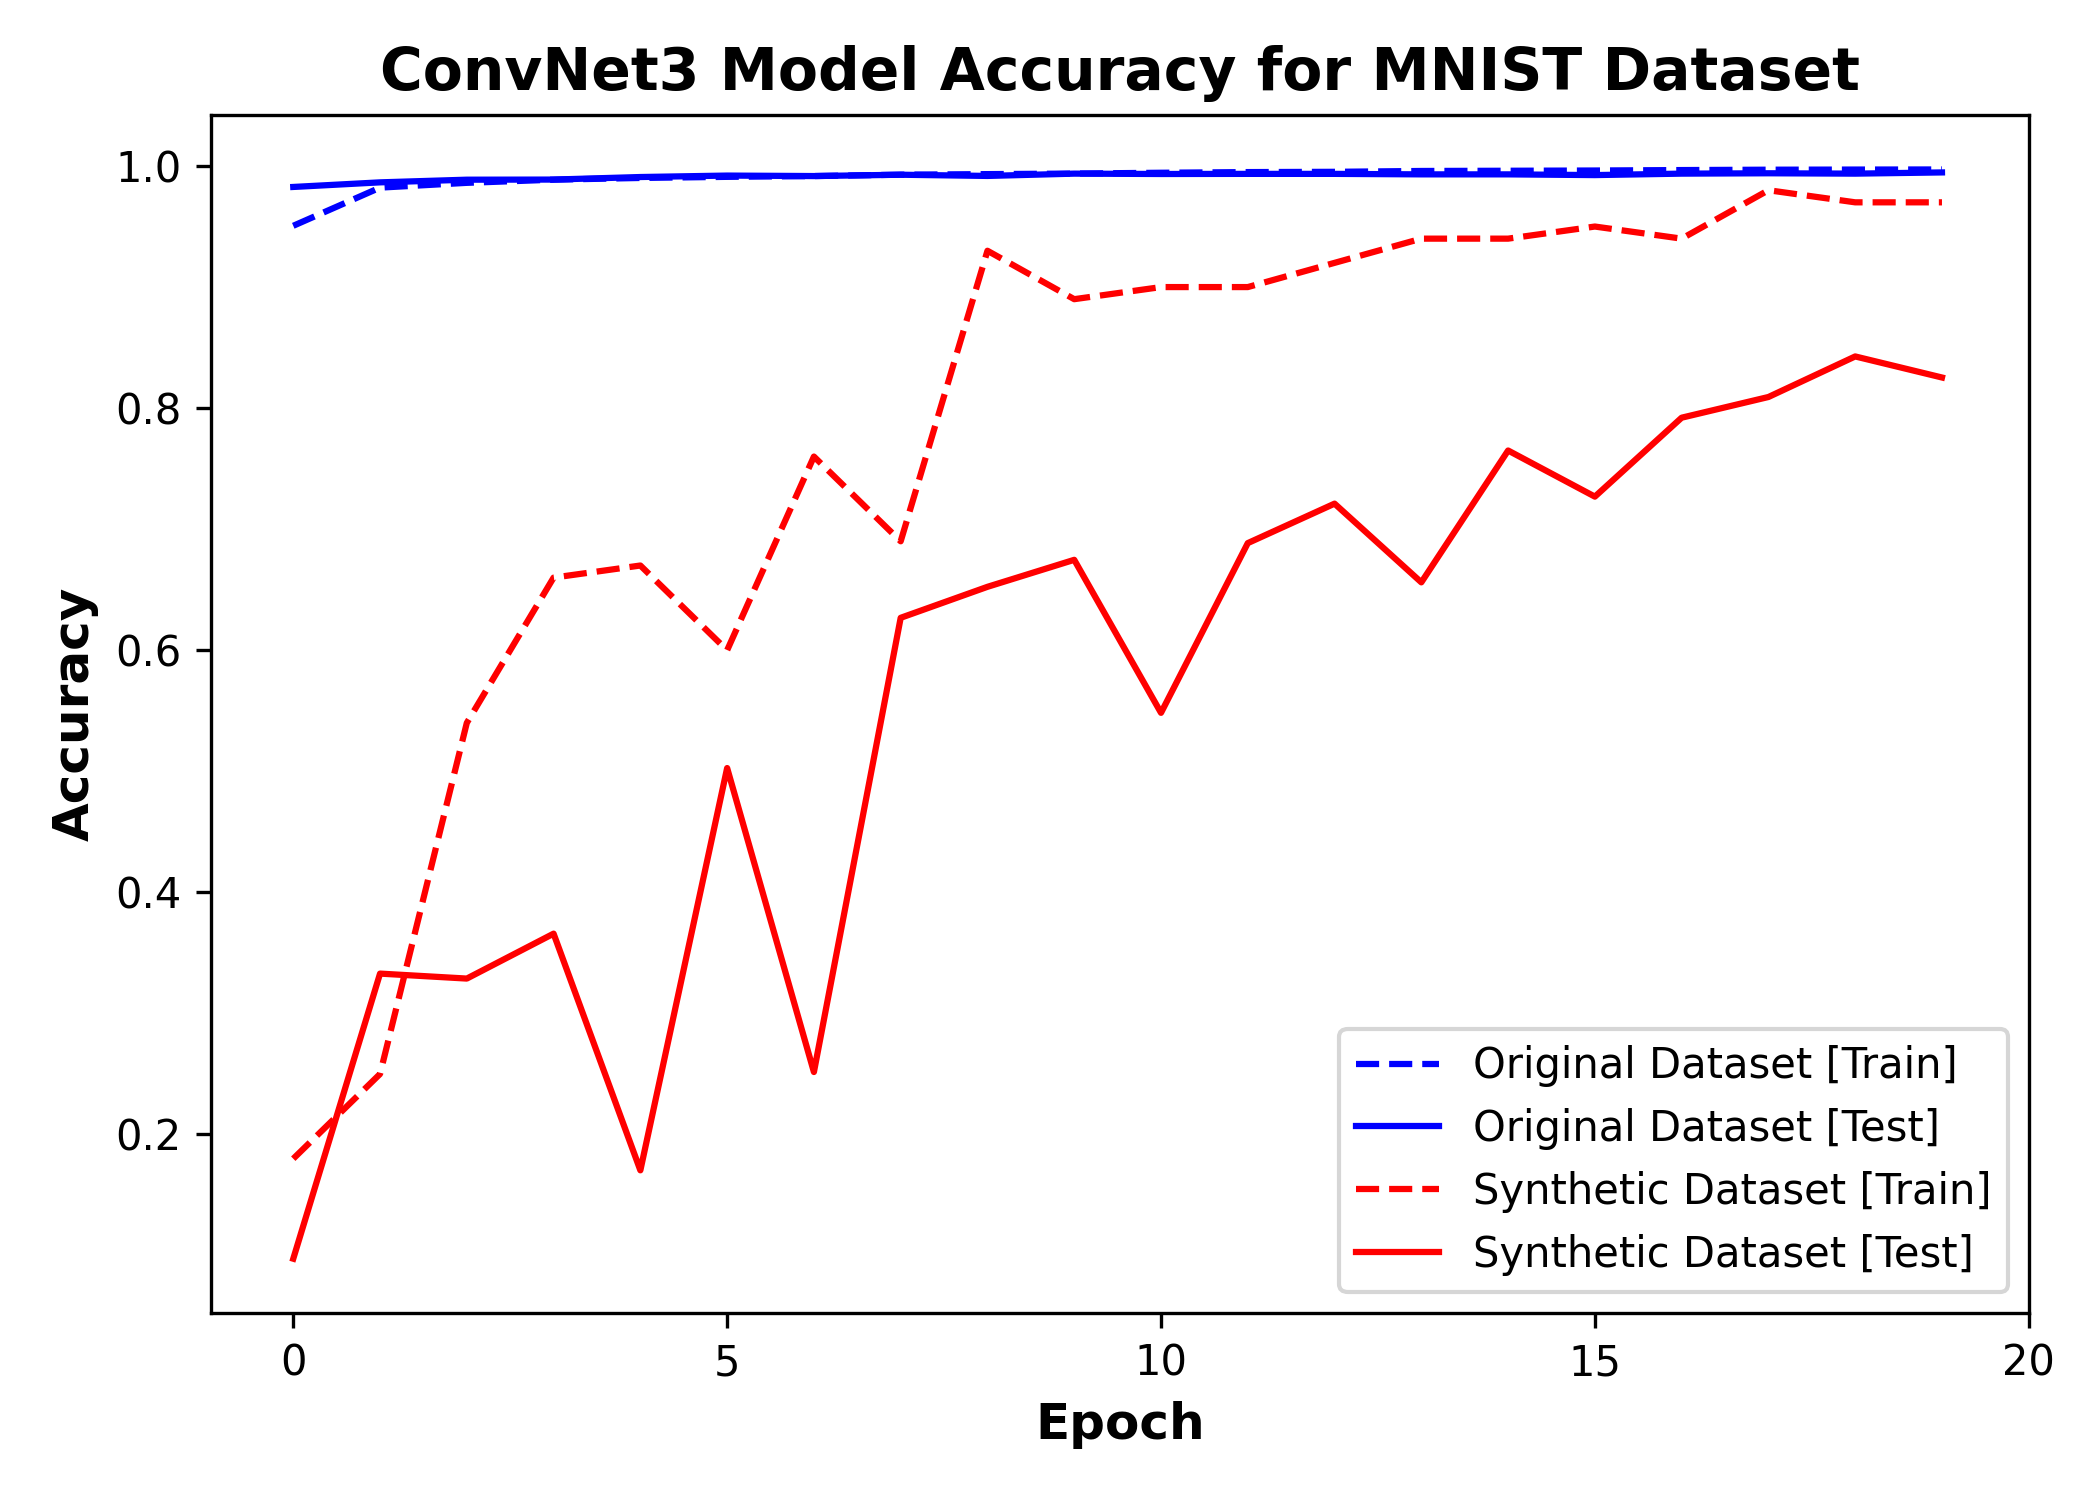
\includegraphics[width=\textwidth]{../report/figures/mnist_syn_acc.png}

				\end{minipage}
				\hfill
				% Second image
				\begin{minipage}{0.48\textwidth}
					\centering
					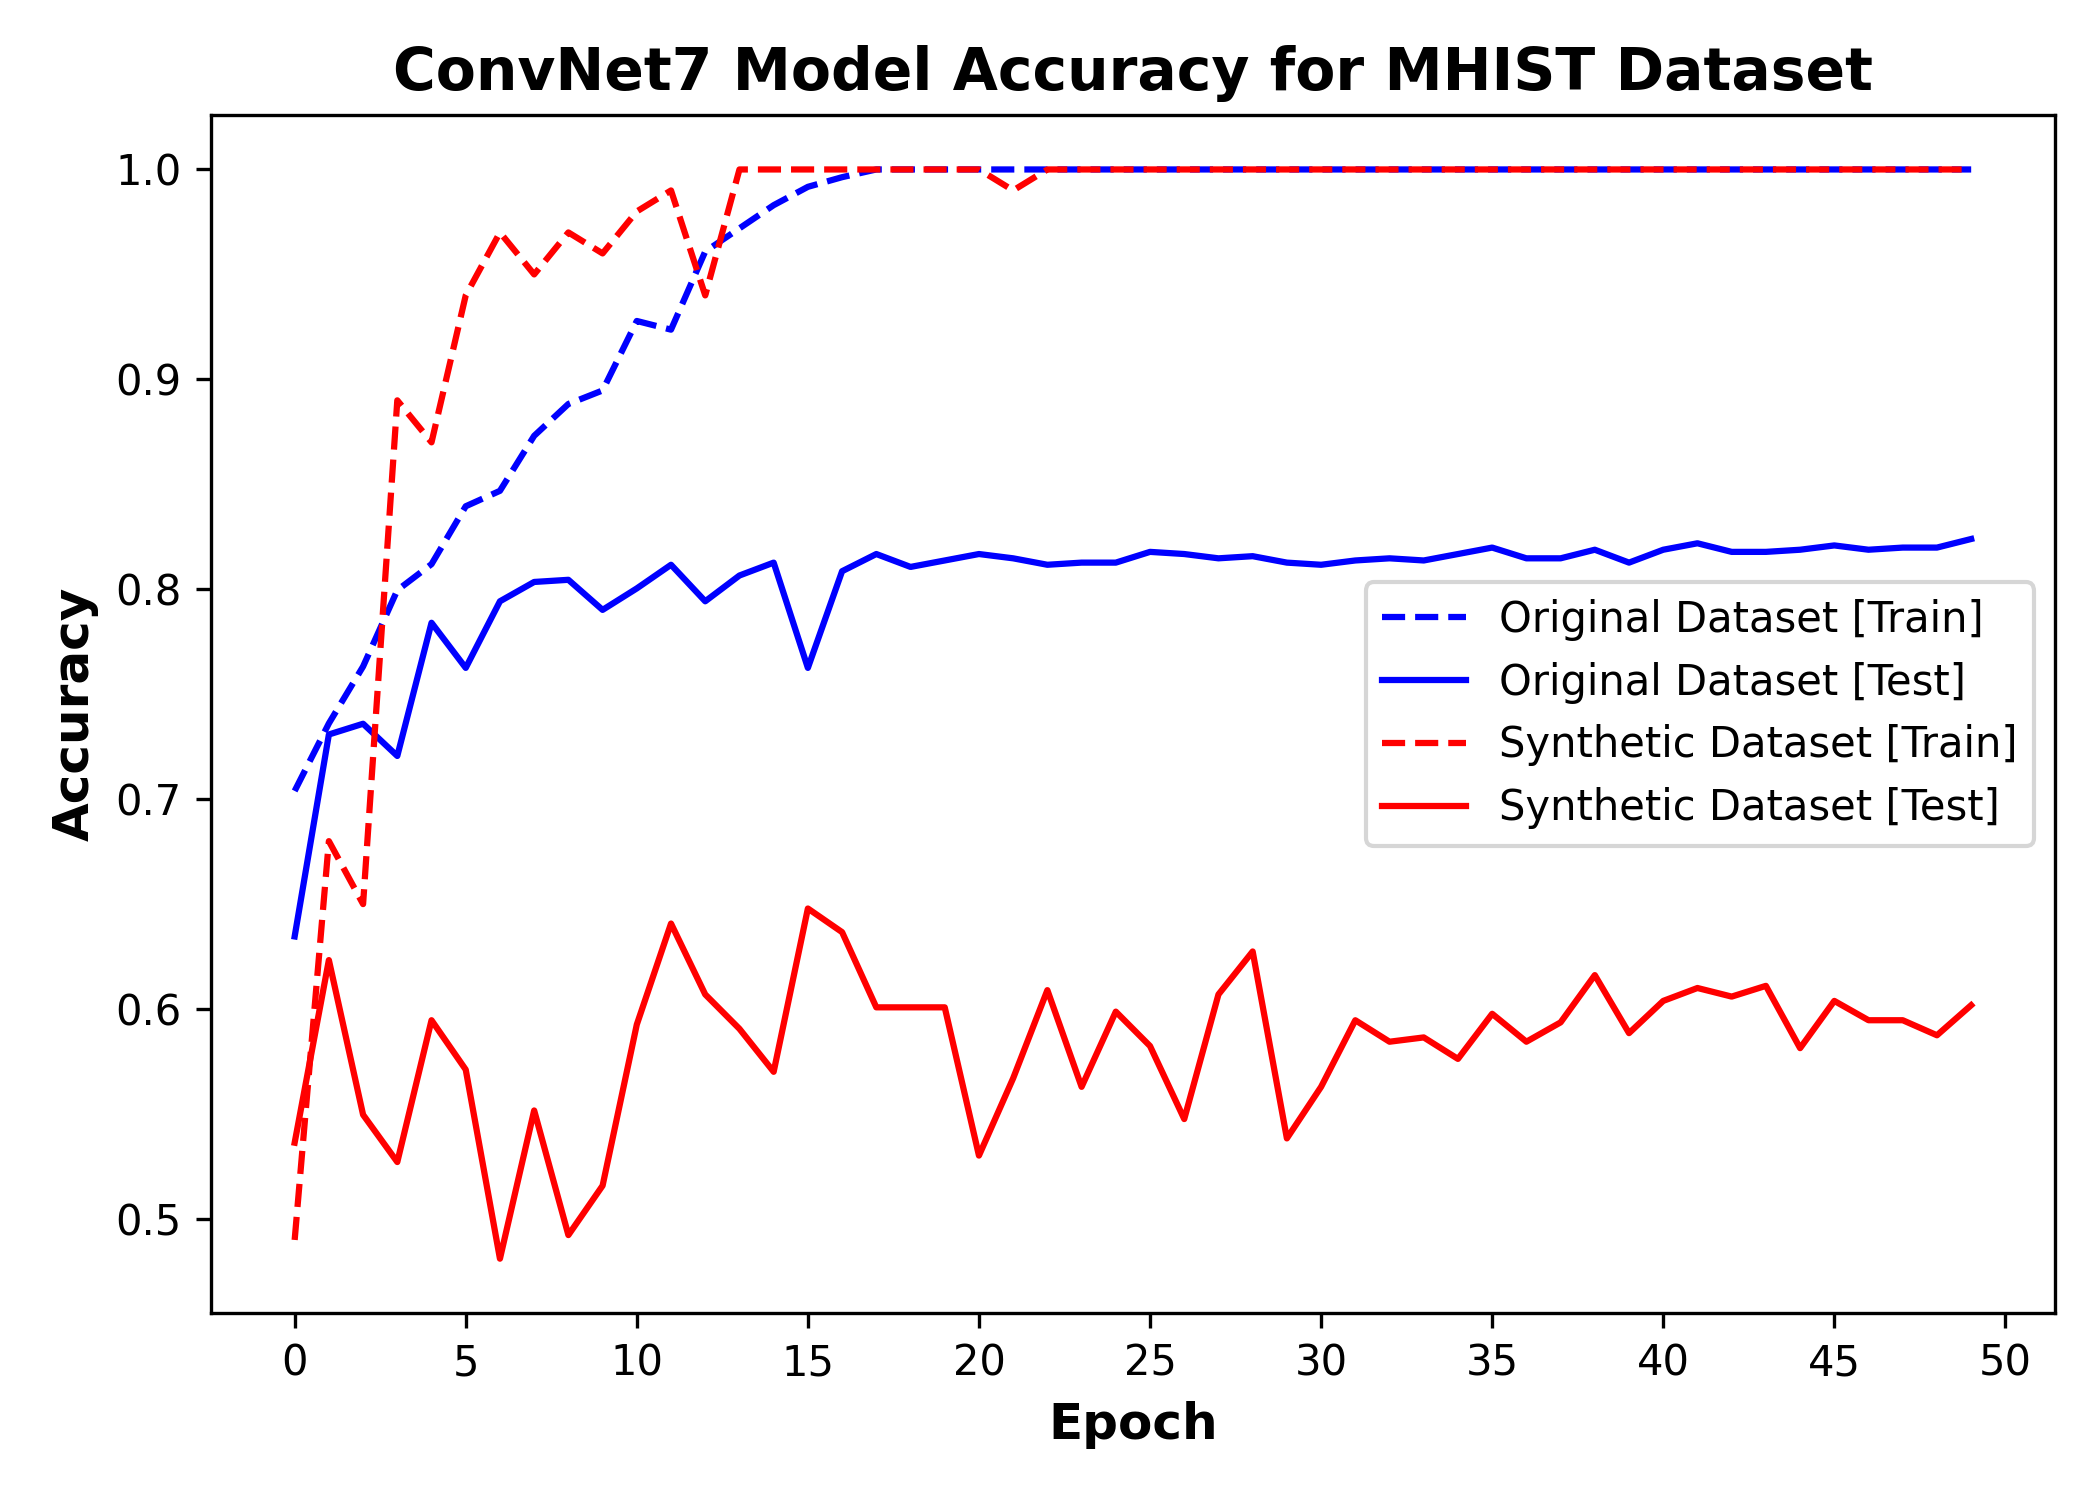
\includegraphics[width=\textwidth]{../report/figures/mhist_syn_acc.png}

				\end{minipage}

			\end{figure}
			
			\begin{figure}[ht]
				\centering
				% First image
				\begin{minipage}{0.48\textwidth}
					\centering
					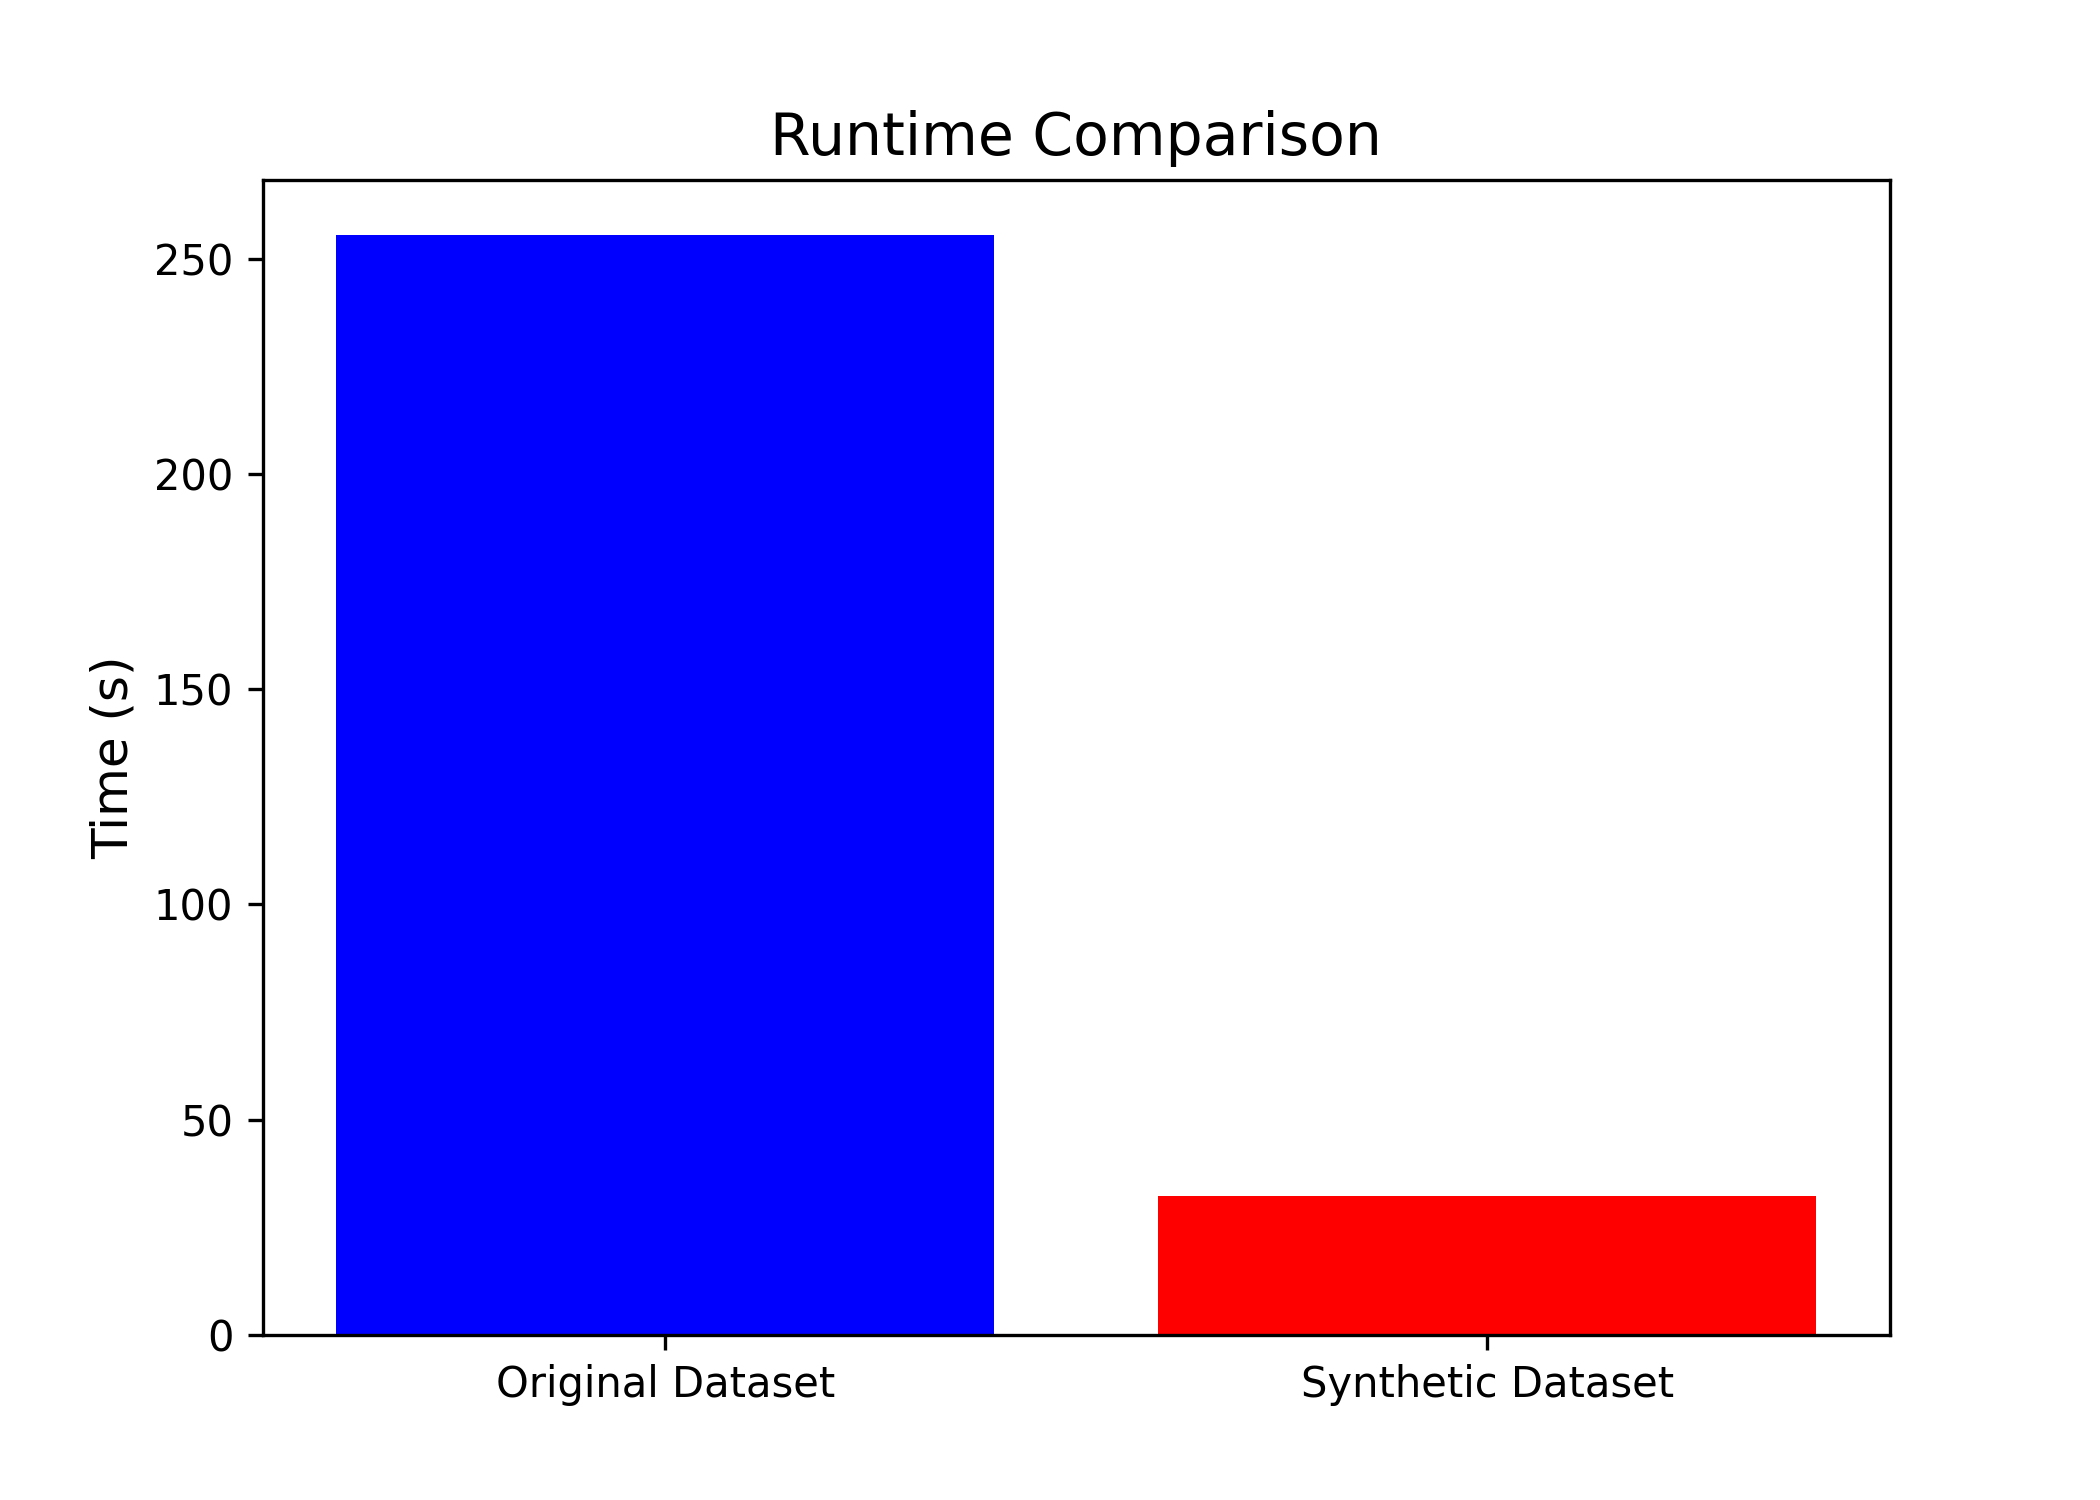
\includegraphics[width=\textwidth]{../report/figures/mnist_syn_time.png}
					
				\end{minipage}
				\hfill
				% Second image
				\begin{minipage}{0.48\textwidth}
					\centering
					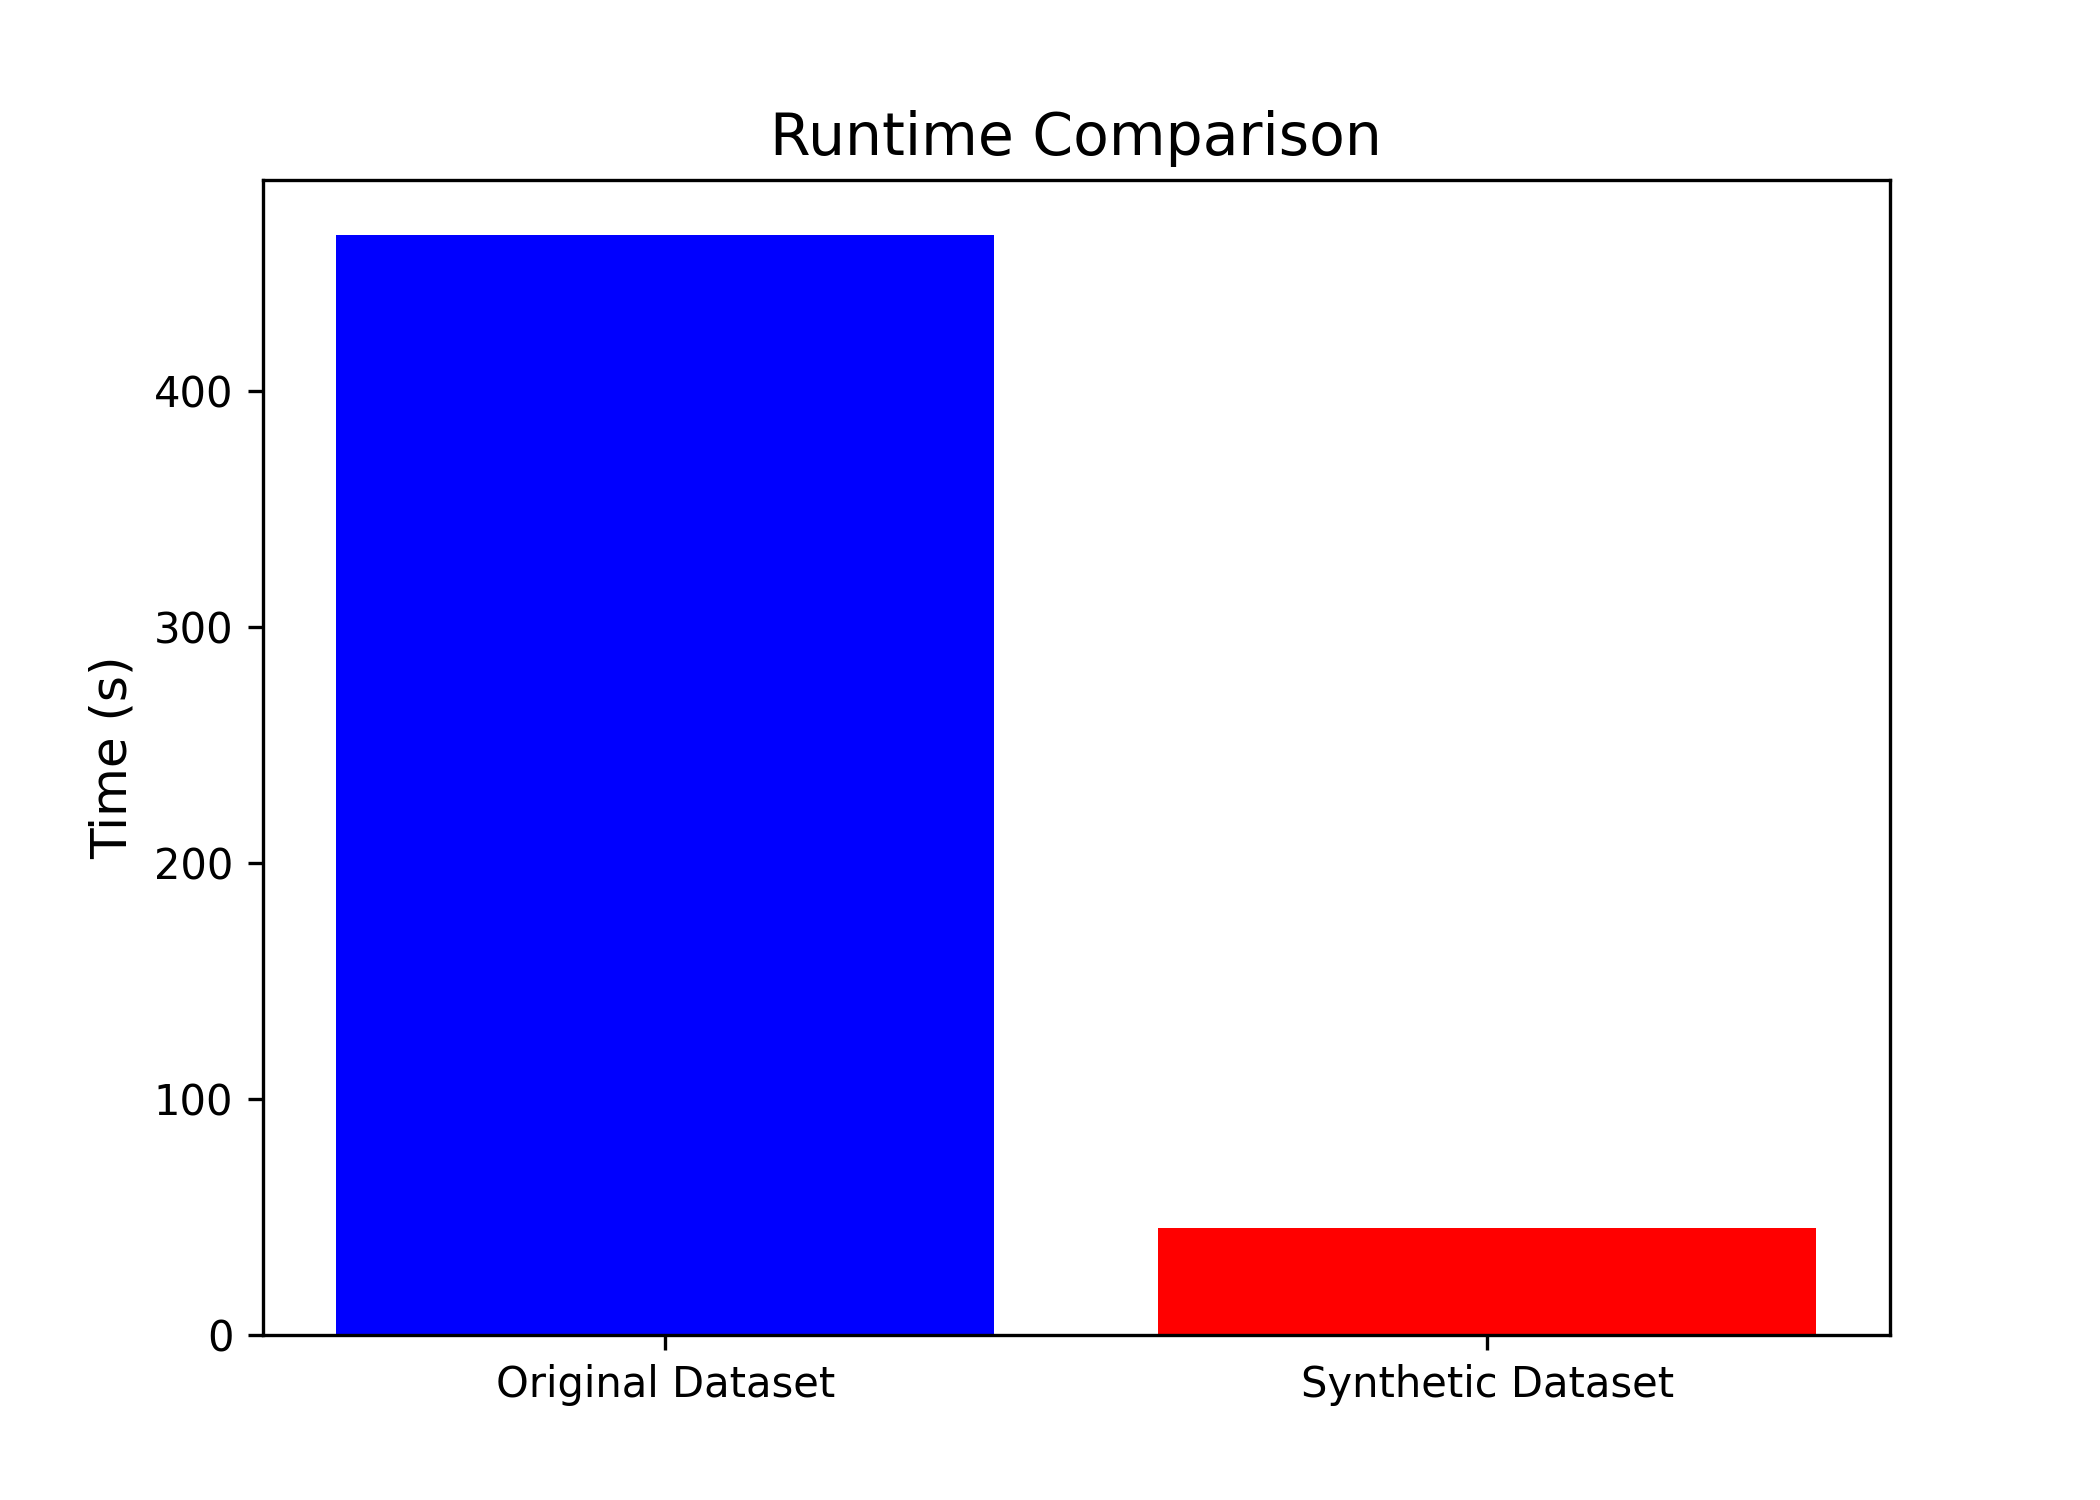
\includegraphics[width=\textwidth]{../report/figures/mhist_syn_time.png}
					
				\end{minipage}
				
			\end{figure}
			
		\end{block}
		
		\begin{block}{Cross-Architecture Generalization}
			
			\begin{figure}[ht]
				\centering
				% First image
				\begin{minipage}{0.48\textwidth}
					\centering
					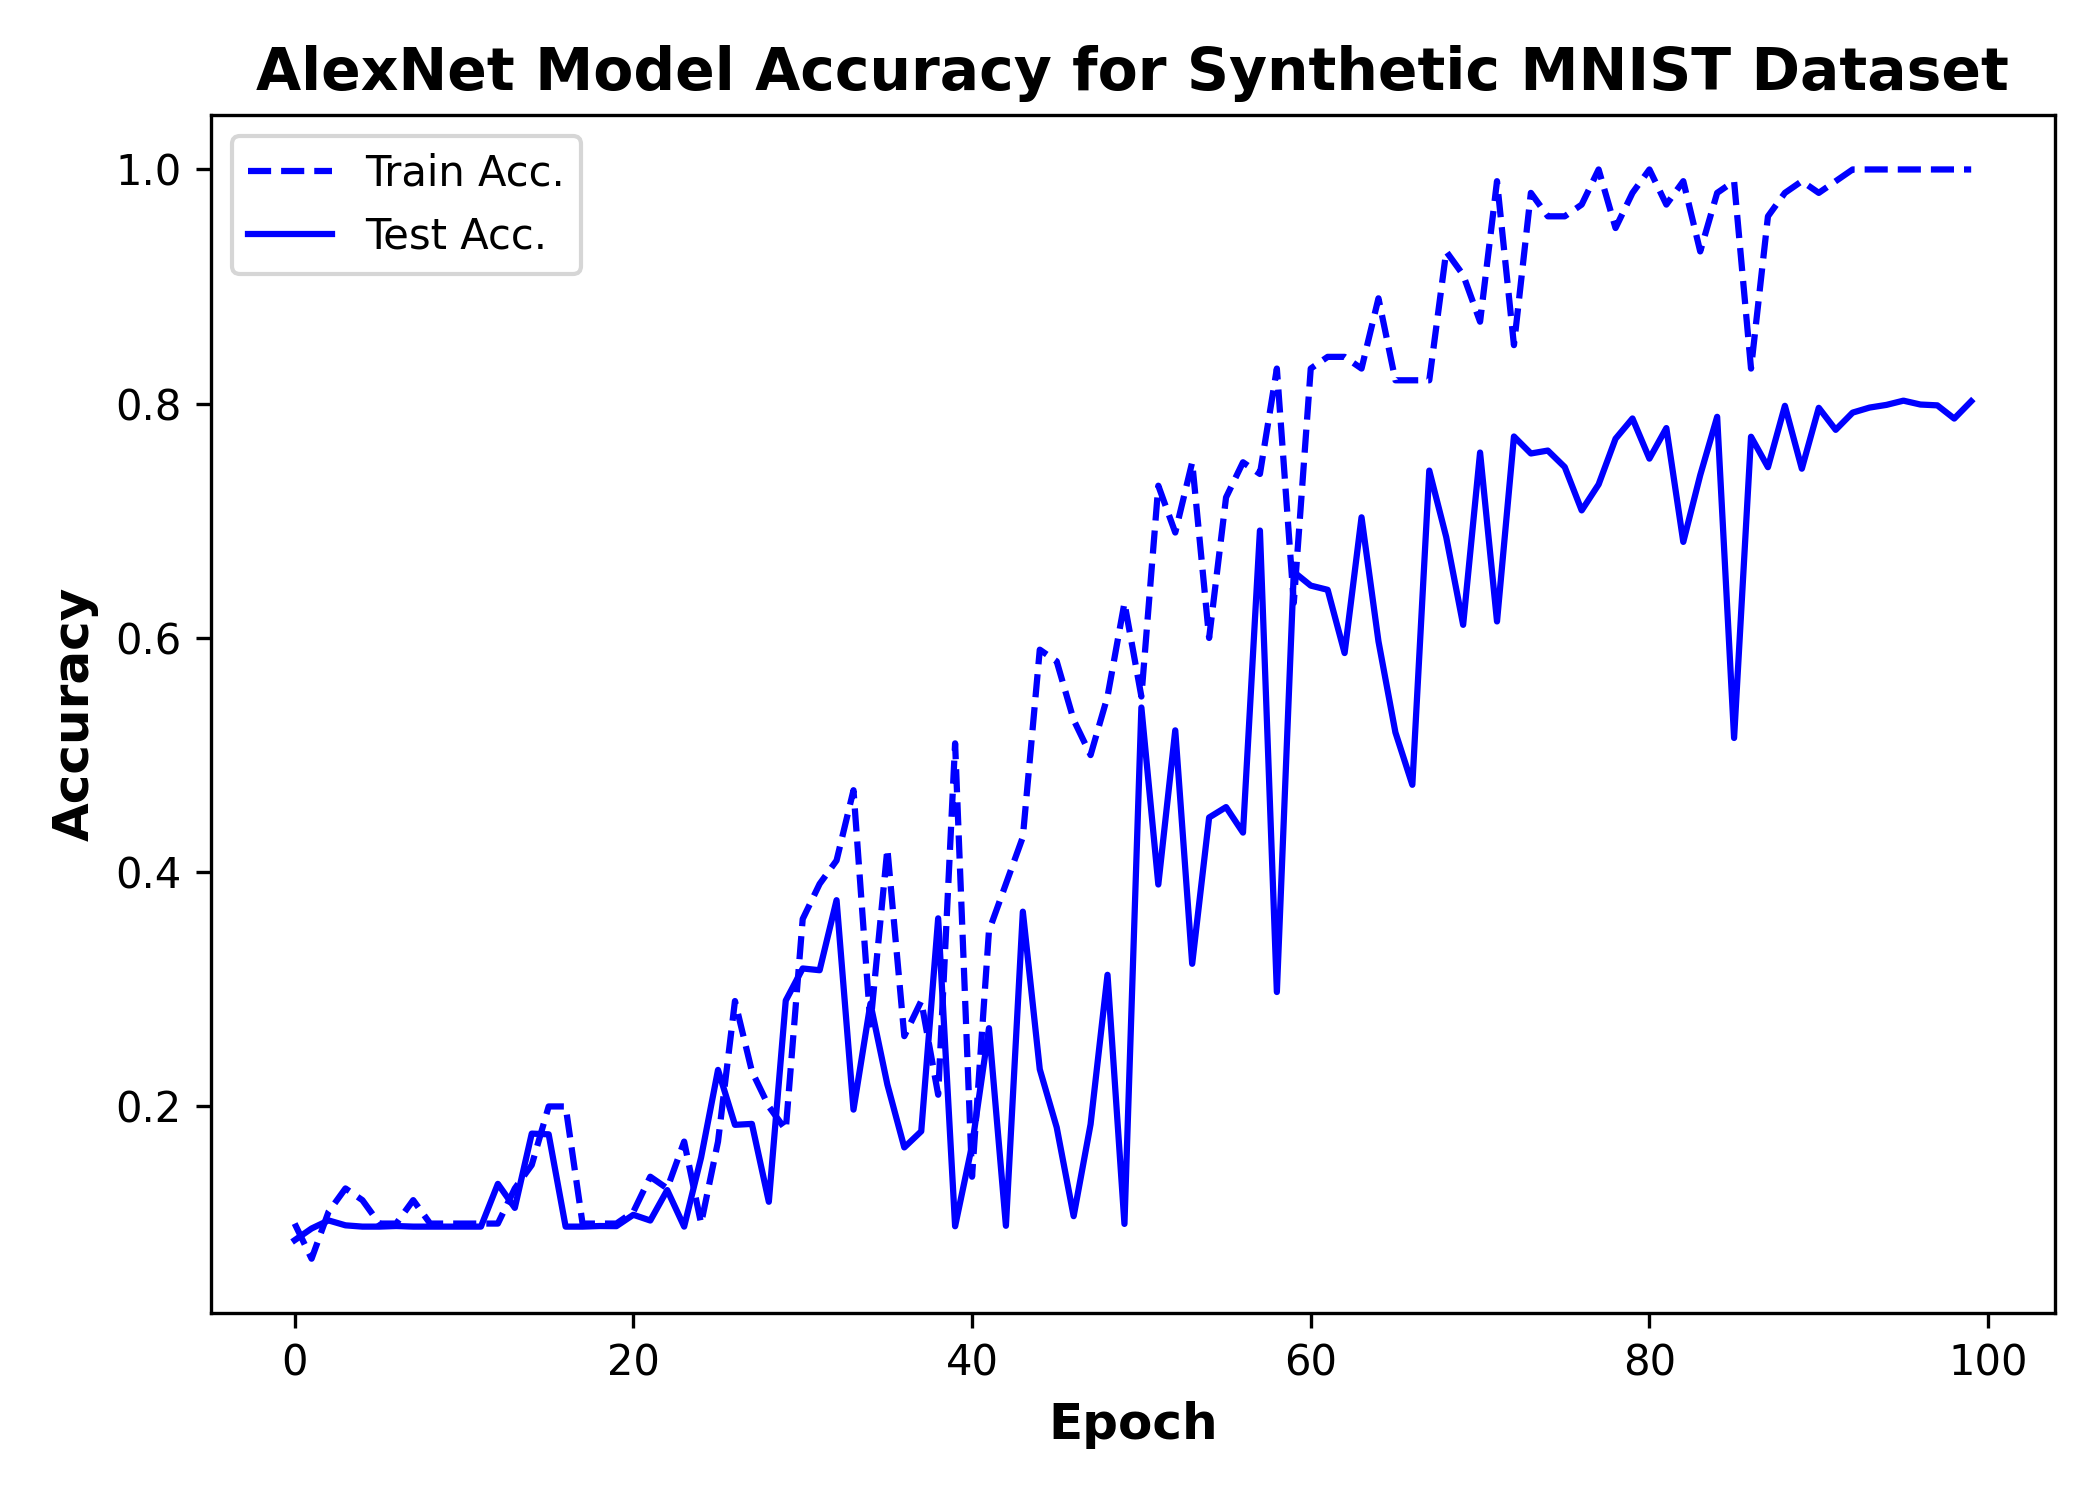
\includegraphics[width=\textwidth]{../report/figures/mnist_alex_acc.png}
					
				\end{minipage}
				\hfill
				% Second image
				\begin{minipage}{0.48\textwidth}
					\centering
					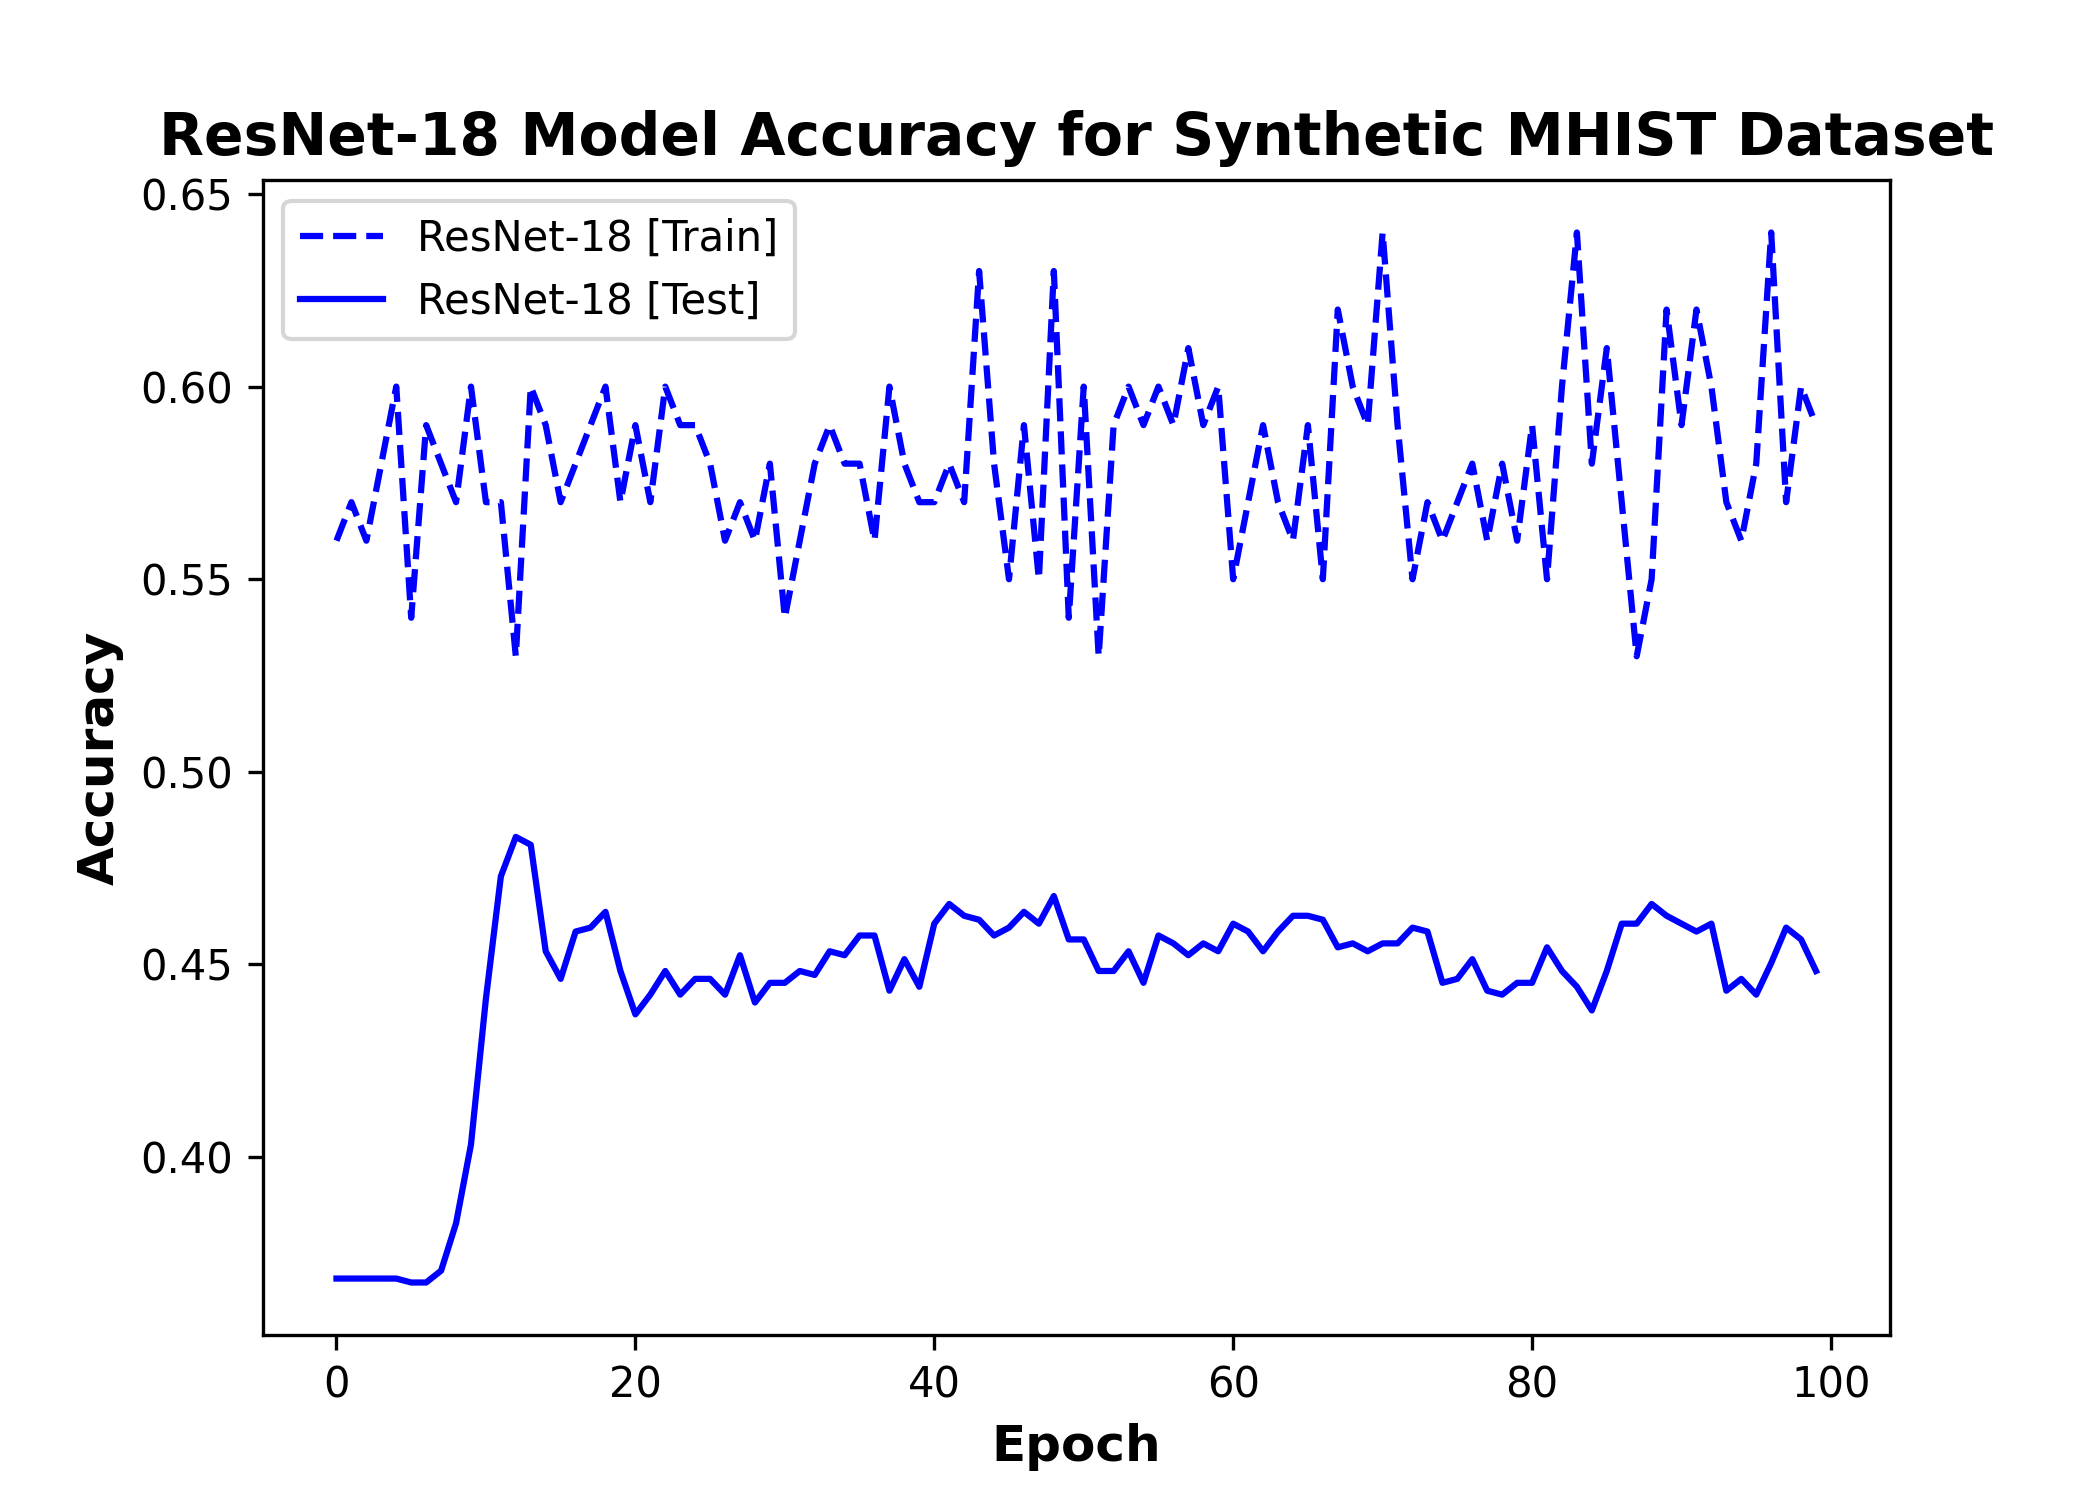
\includegraphics[width=\textwidth]{../report/figures/mhist_resnet_acc.png}
					
				\end{minipage}
				
			\end{figure}
			
		\end{block}

	\end{column}
	\separatorcolumn
	\begin{column}{\colwidth}
		\begin{block}{Prioritize Alignment in Dataset Distillation}
			\begin{columns}
				\begin{column}{0.5\textwidth}
					\textbf{Synthetic Dataset Generation:}  
					The figure showcases synthetic images generated with DataDAM, demonstrating the retention of critical dataset features in compact forms. While visually different from the original, these images effectively train models with reduced computational costs.  
				\end{column}
				\begin{column}{0.5\textwidth}
					\begin{figure}
						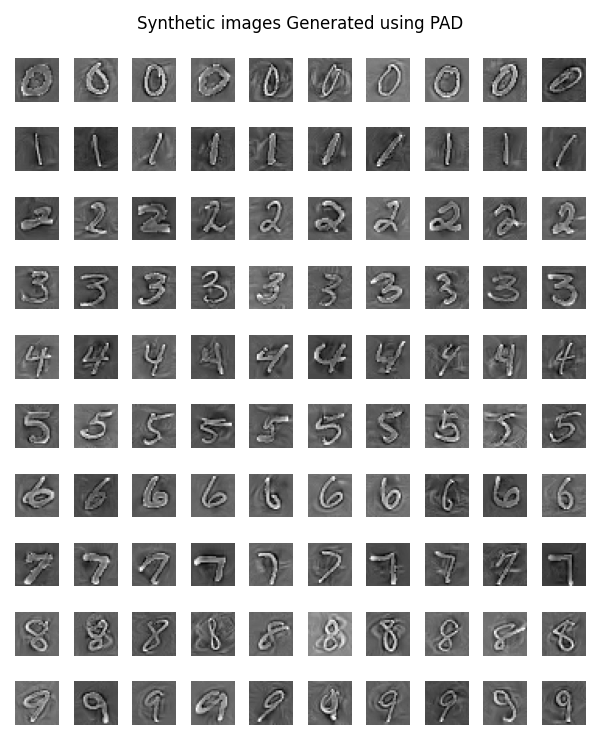
\includegraphics[width=\linewidth]{../report/figures/synthetic_images_task2.png}
					\end{figure}
				\end{column}

			\end{columns}
			
			\begin{figure}[ht]
				\centering
				% First image
				\begin{minipage}{0.48\textwidth}
					\centering
					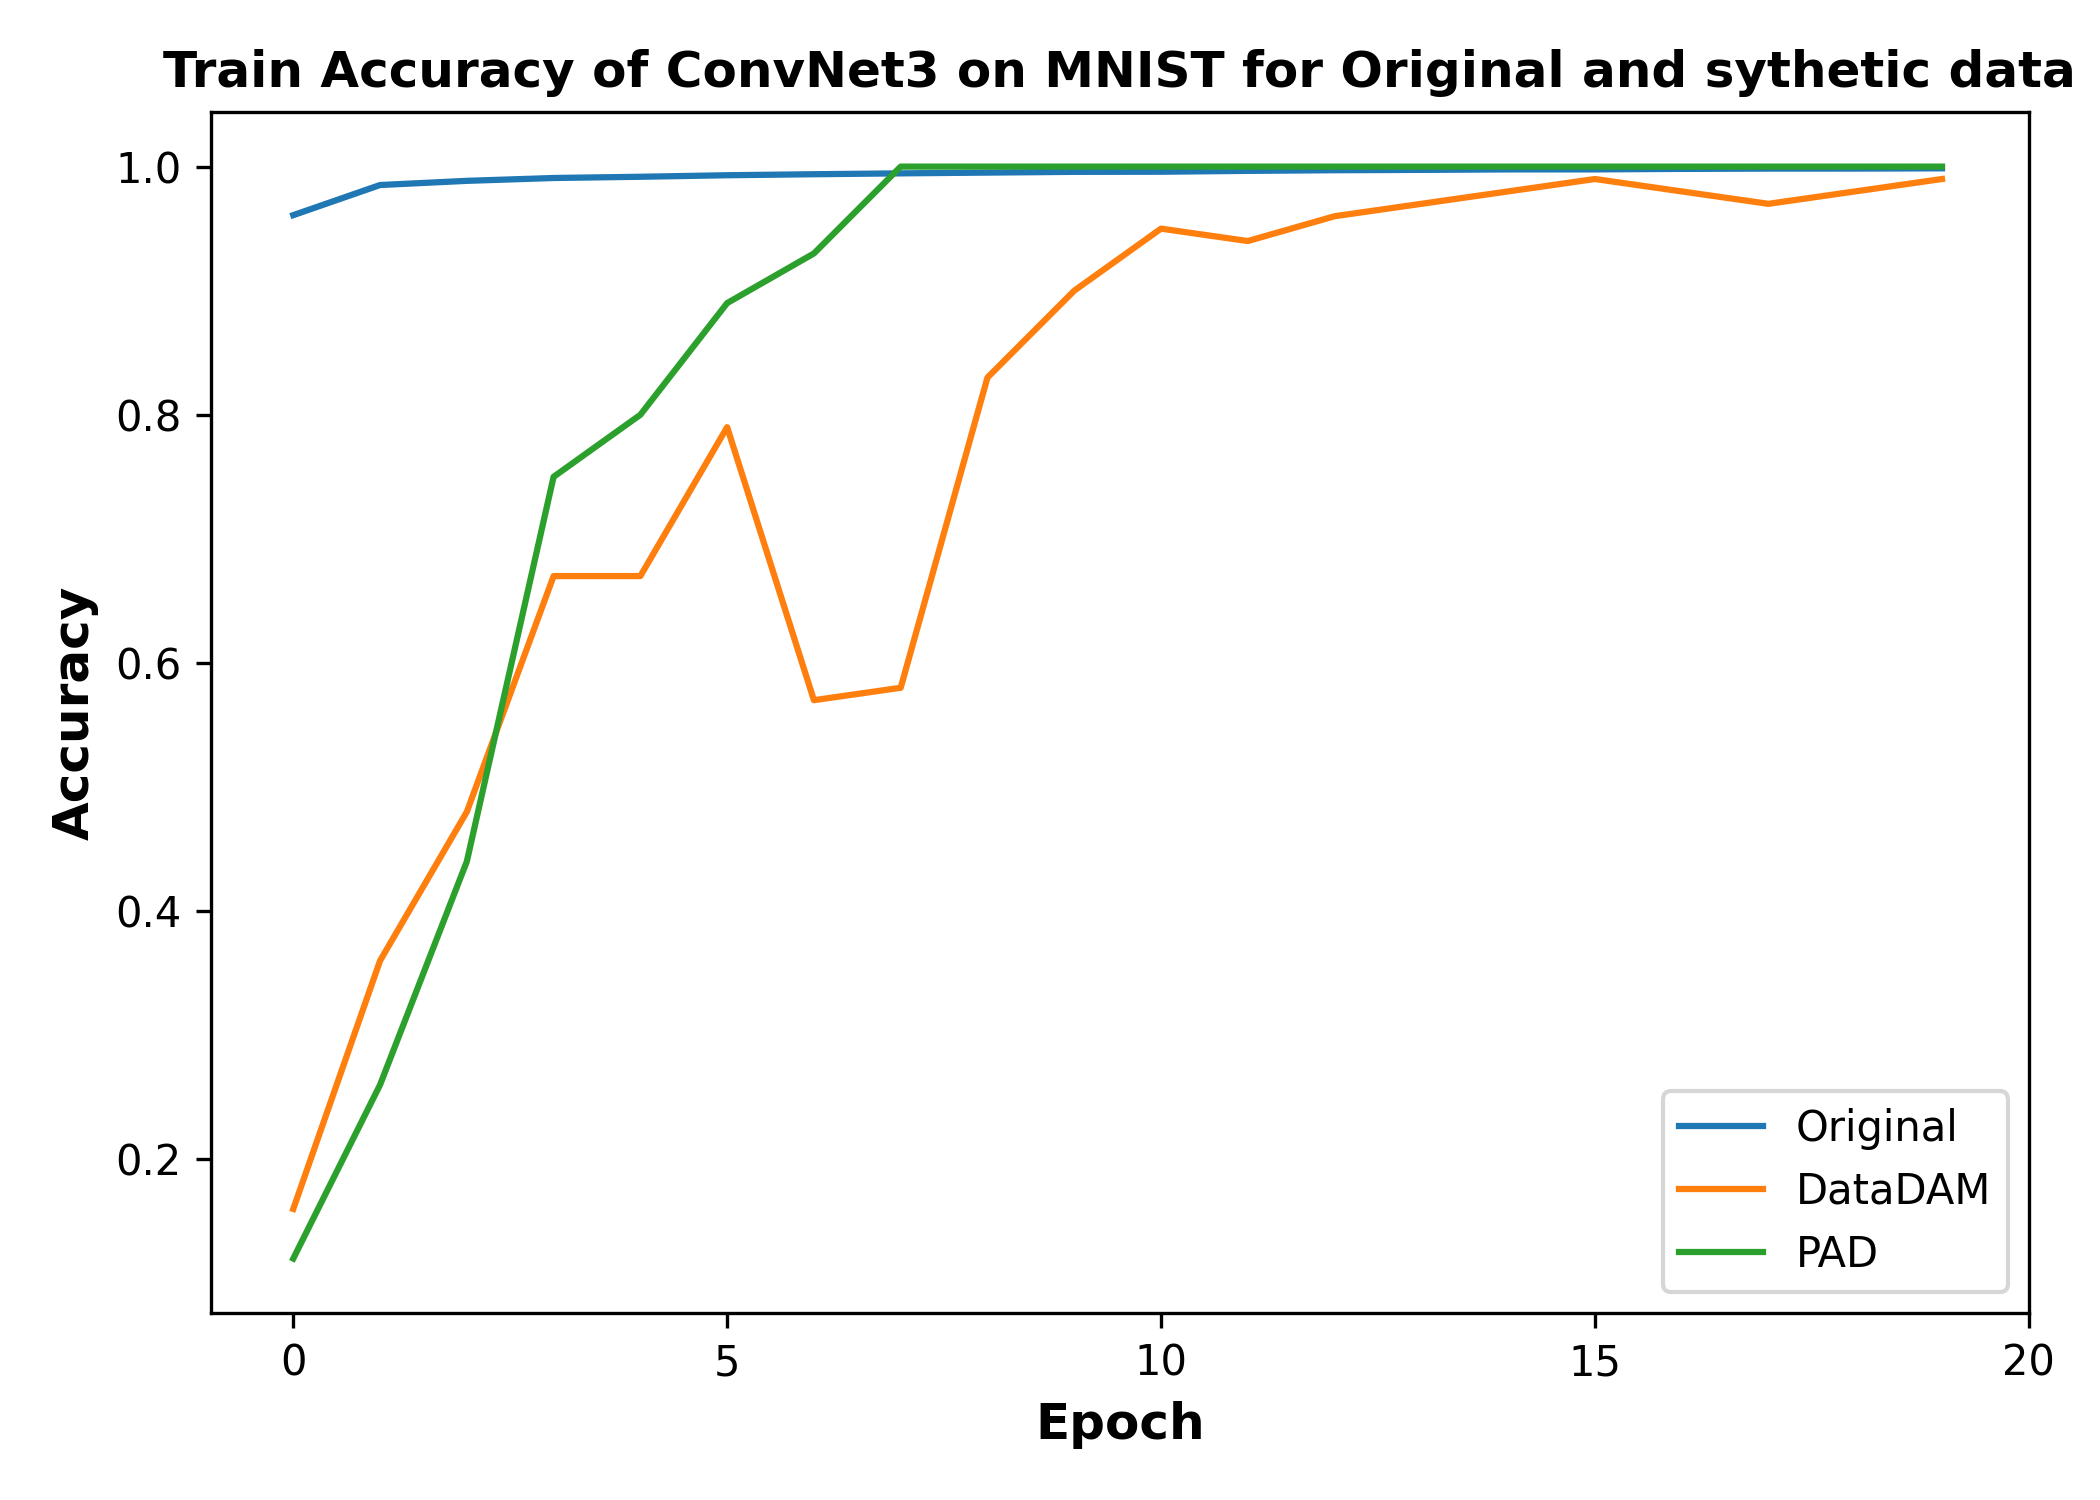
\includegraphics[width=\textwidth]{../report/figures/train_acc_task2.png}
					
				\end{minipage}
				\hfill
				% Second image
				\begin{minipage}{0.48\textwidth}
					\centering
					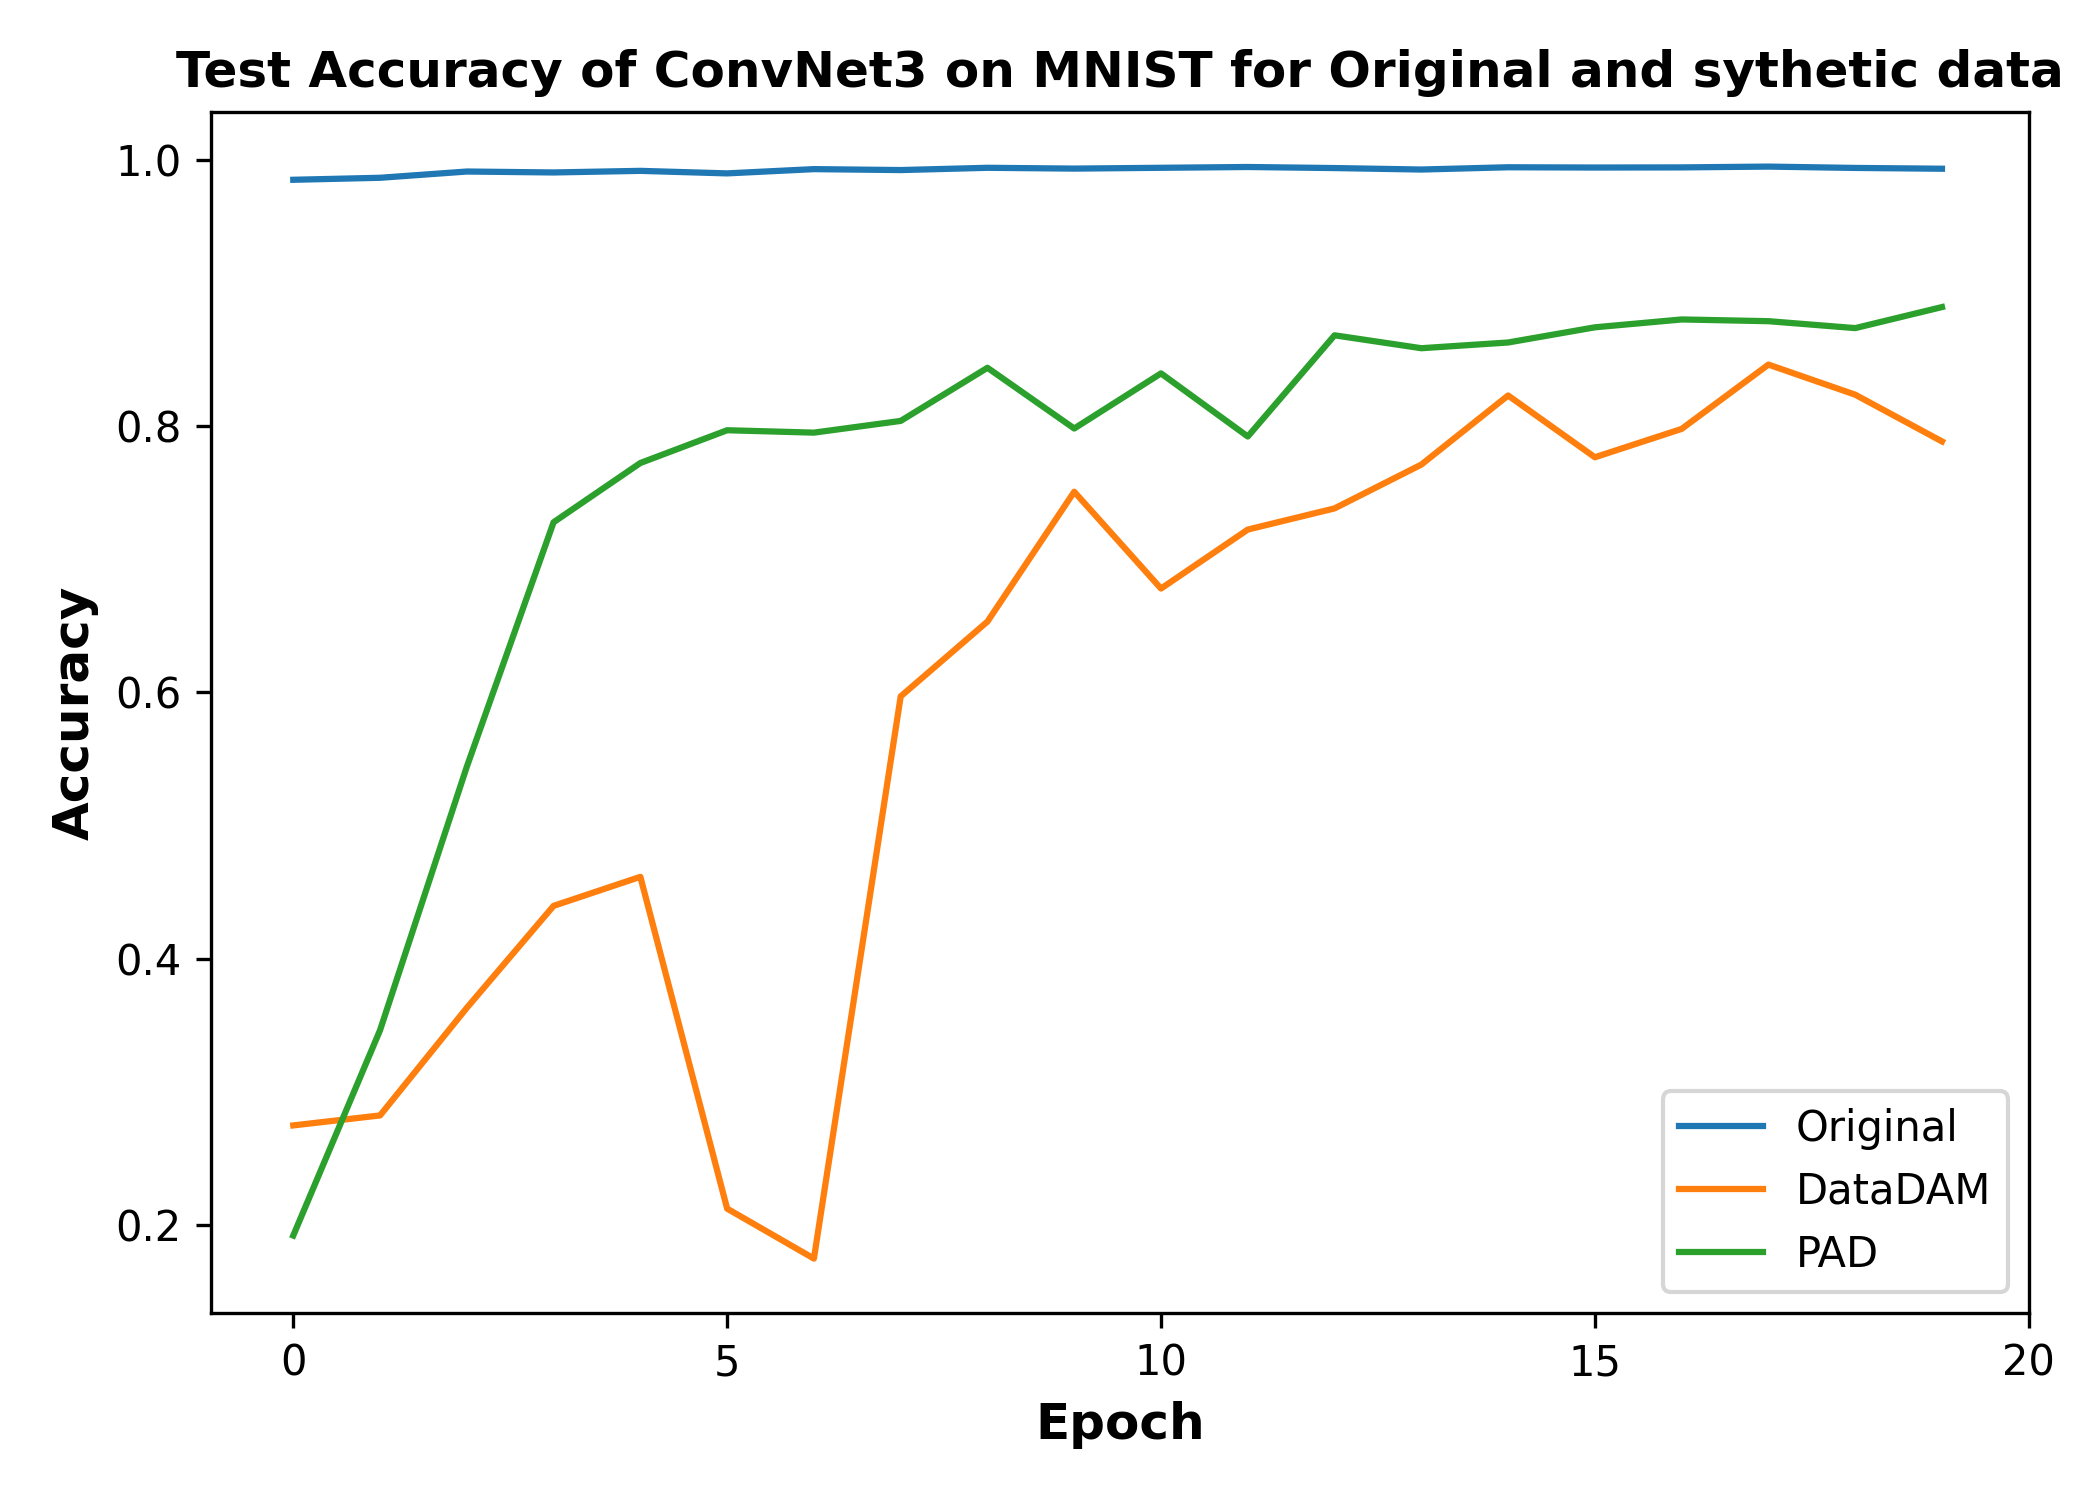
\includegraphics[width=\textwidth]{../report/figures/test_acc_task2.png}
					
				\end{minipage}
				
			\end{figure}
			
		\begin{block}{Applications}
			\begin{itemize}
				\item \textbf{Neural Architecture Search (NAS)} Provides proxy datasets for rapid exploration of architectures.
				\item \textbf{Privacy Preservation} Limits exposure to sensitive information by condensing data into unidentifiable formats.
			\end{itemize}
		\end{block}
			
		\end{block}
		\begin{block}{References}
			
			\nocite{*}
			\footnotesize{\bibliographystyle{plain}\bibliography{poster}}
			
		\end{block}
	\end{column}
\end{columns}
\end{document}



